%% Copernicus Publications Manuscript Preparation Template for LaTeX Submissions
%% ---------------------------------
%% This template should be used for copernicus.cls
%% The class file and some style files are bundled in the Copernicus Latex Package, which can be downloaded from the different journal webpages.
%% For further assistance please contact Copernicus Publications at: production@copernicus.org
%% https://publications.copernicus.org/for_authors/manuscript_preparation.html


%% Please use the following documentclass and journal abbreviations for discussion papers and final revised papers.

%% 2-column papers and discussion papers
\documentclass[essd, manuscript]{copernicus}

\usepackage[default, scale=0.95]{opensans}
\usepackage[section]{placeins}
\usepackage{amsmath}
\usepackage[final]{pdfpages}
\usepackage{lscape}
\usepackage{longtable}
\usepackage{booktabs}

%% Journal abbreviations (please use the same for discussion papers and final revised papers)


% Advances in Geosciences (adgeo)
% Advances in Radio Science (ars)
% Advances in Science and Research (asr)
% Advances in Statistical Climatology, Meteorology and Oceanography (ascmo)
% Annales Geophysicae (angeo)
% Archives Animal Breeding (aab)
% ASTRA Proceedings (ap)
% Atmospheric Chemistry and Physics (acp)
% Atmospheric Measurement Techniques (amt)
% Biogeosciences (bg)
% Climate of the Past (cp)
% DEUQUA Special Publications (deuquasp)
% Drinking Water Engineering and Science (dwes)
% Earth Surface Dynamics (esurf)
% Earth System Dynamics (esd)
% Earth System Science Data (essd)
% E&G Quaternary Science Journal (egqsj)
% Fossil Record (fr)
% Geochronology (gchron)
% Geographica Helvetica (gh)
% Geoscience Communication (gc)
% Geoscientific Instrumentation, Methods and Data Systems (gi)
% Geoscientific Model Development (gmd)
% History of Geo- and Space Sciences (hgss)
% Hydrology and Earth System Sciences (hess)
% Journal of Micropalaeontology (jm)
% Journal of Sensors and Sensor Systems (jsss)
% Mechanical Sciences (ms)
% Natural Hazards and Earth System Sciences (nhess)
% Nonlinear Processes in Geophysics (npg)
% Ocean Science (os)
% Primate Biology (pb)
% Proceedings of the International Association of Hydrological Sciences (piahs)
% Scientific Drilling (sd)
% SOIL (soil)
% Solid Earth (se)
% The Cryosphere (tc)
% Web Ecology (we)
% Wind Energy Science (wes)


%% \usepackage commands included in the copernicus.cls:
%\usepackage[german, english]{babel}
%\usepackage{tabularx}
%\usepackage{cancel}
%\usepackage{multirow}
%\usepackage{supertabular}
%\usepackage{algorithmic}
%\usepackage{algorithm}
%\usepackage{amsthm}
%\usepackage{float}
%\usepackage{subfig}
%\usepackage{rotating}

\DeclareUnicodeCharacter{2212}{-}

\makeatother
\makeatletter
\renewcommand\paragraph{\@startsection{paragraph}{4}{\z@}%
                                     {-3.25ex\@plus -1ex \@minus -.2ex}%
                                     {1.5ex \@plus .2ex}%
                                     {\normalfont\normalsize\bfseries}}
% number \paragraph
\setcounter{secnumdepth}{4}


%\usepackage{hyperref}


\begin{document}

\title{The Malina oceanographic expedition: How do changes in ice cover, permafrost and UV radiation impact biodiversity and biogeochemical fluxes in the Arctic Ocean?}

% \Author[affil]{given_name}{surname}

\Author[1]{Philippe}{Massicotte}
\Author[2,3]{Rainer}{Amon}
\Author[4,5]{David}{Antoine}
\Author[6]{Philippe}{Archambault}
\Author[7,8,9]{Sergio}{Balzano}
\Author[10]{Simon}{Bélanger}
\Author[11,12]{Ronald}{Benner}
\Author[7]{Dominique}{Boeuf}
\Author[5]{Annick}{Bricaud}
\Author[1]{Flavienne}{Bruyant}
\Author[13]{Gwenaëlle}{Chaillou}
\Author[14]{Malik}{Chami}
\Author[15]{Bruno}{Charrière}
\Author[16]{Jingan}{Chen}
\Author[5]{Hervé}{Claustre}
\Author[1]{Pierre}{Coupel}
\Author[15]{Nicole}{Delsaut}
\Author[5]{David}{Doxaran}
\Author[17]{Jens}{Ehn}
\Author[18]{Cédric}{Fichot}
\Author[1]{Marie-Hélène}{Forget}
\Author[19]{Pingqing}{Fu}
\Author[1]{Jonathan}{Gagnon}
\Author[20]{Nicole}{Garcia}
\Author[21]{Beat}{Gasser}
\Author[22]{Jean-François}{Ghiglione}
\Author[5]{Gaby}{Gorsky}
\Author[13]{Michel}{Gosselin}
\Author[23]{Priscillia}{Gourvil}
\Author[24]{Yves}{Gratton}
\Author[13]{Pascal}{Guillot}
\Author[25]{Hermann J.}{Heipieper}
\Author[15]{Serge}{Heussner}
\Author[26]{Stanford B.}{Hooker}
\Author[27]{Yannick}{Huot}
\Author[7]{Christian}{Jeanthon}
\Author[28]{Wade}{Jeffrey}
\Author[22]{Fabien}{Joux}
\Author[29]{Kimitaka}{Kawamura}
\Author[30]{Bruno}{Lansard}
\Author[5]{Edouard}{Leymarie}
\Author[31]{Heike}{Link}
\Author[1]{Connie}{Lovejoy}
\Author[1,32]{Claudie}{Marec}
\Author[7]{Dominique}{Marie}
\Author[1]{Johannie}{Martin}
\Author[1,33]{Guillaume}{Massé}
\Author[1]{Atsushi}{Matsuoka}
\Author[34]{Vanessa}{McKague}
\Author[5,35]{Alexandre}{Mignot}
\Author[36]{William L.}{Miller}
\Author[21]{Juan-Carlos}{Miquel}
\Author[37]{Alfonso}{Mucci}
\Author[38]{Kaori}{Ono}
\Author[22]{Eva}{Ortega-Retuerta}
\Author[20]{Christos}{Panagiotopoulos}
\Author[17]{Tim}{Papakyriakou}
\Author[5]{Marc}{Picheral}
\Author[39,40]{Dieter}{Piepenburg}
\Author[5]{Louis}{Prieur}
\Author[20]{Patrick}{Raimbault}
\Author[5]{Joséphine}{Ras}
\Author[41]{Rick A.}{Reynolds}
\Author[13]{André}{Rochon}
\Author[20]{Jean-François}{Rontani}
\Author[42]{Catherine}{Schmechtig}
\Author[43]{Sabine}{Schmidt}
\Author[20]{Richard}{Sempéré}
\Author[11,44]{Yuan}{Shen}
\Author[45,46]{Guisheng}{Song}
\Author[41]{Dariusz}{Stramski}
\Author[47]{Dave}{Stroud G.}
\Author[38]{Eri}{Tachibana}
\Author[5]{Alexandre}{Thirouard}
\Author[21]{Imma}{Tolosa}
\Author[1]{Jean-Éric}{Tremblay}
\Author[48]{Mickael}{Vaïtilingom}
\Author[7,49]{Daniel}{Vaulot}
\Author[20]{Frédéric}{Vaultier}
\Author[50]{John K.}{Volkman}
\Author[51]{Jorien E.}{Vonk}
\Author[13]{Huixiang}{Xie}
\Author[41,52,53]{Guangming}{Zheng}
\Author[1]{Marcel}{Babin}
    
\affil[1]{Takuvik Joint International Laboratory / UMI 3376, ULAVAL (Canada) - CNRS (France), Université Laval, Québec, QC, Canada}
\affil[2]{Department of Marine and Coastal Environmental Science, Texas A\&M University Galveston Campus, Galveston, Texas, 77553, USA}
\affil[3]{Department of Oceanography, Texas A\&M University, College Station, Texas, 77843, USA}
\affil[4]{Remote Sensing and Satellite Research Group, School of Earth and Planetary Sciences, Curtin University, Perth, WA 6845, Australia}
\affil[5]{Sorbonne Université, CNRS, Laboratoire d’Océanographie de Villefranche (LOV) / UMR 7093, F-06230 Villefranche-sur-Mer, France}
\affil[6]{ArcticNet, Québec-Océan, Takuvik Joint International Laboratory / UMI 3376, ULAVAL (Canada) - CNRS (France), Université Laval, Québec, QC, Canada}
\affil[7]{Sorbonne Université, CNRS, Station Biologique de Roscoff - Adaptation et Diversité en Milieu Marin / UMR 7144, 29680 Roscoff, France}
\affil[8]{Present address: Stazione Zoologica Anton Dohrn Napoli (SZN), Naples, Italy}
\affil[9]{NIOZ Royal Netherlands Institute for Sea Research, Den Burg, Netherlands}
\affil[10]{Département de Biologie, Chimie et Géographie (groupes BORÉAS et Québec-Océan), Université du Québec à Rimouski, Rimouski, QC, Canada}
\affil[11]{School of the Earth, Ocean and Environment, University of South Carolina, Columbia, South Carolina, 29208, USA}
\affil[12]{Department of Biological Sciences, University of South Carolina, Columbia, South Carolina, 29208, USA}
\affil[13]{Québec-Océan, Institut des sciences de la mer de Rimouski (ISMER), Université du Québec à Rimouski, Rimouski, QC, Canada}
\affil[14]{Sorbonne Université, CNRS, Laboratoire Atmosphères Milieux Observations Spatiales (LATMOS) / UMR 8190, Boulevard de l’Observatoire, CS 34229, 06304 Nice Cedex, France}
\affil[15]{Université de Perpignan Via Domitia (UPVD), CNRS, Centre de Formation et de Recherche sur les Environnements Méditerranéens (CEFREM) / UMR 5110, 52 Avenue Paul Alduy, 66860 Perpignan Cedex, France}
\affil[16]{SKLEG, Institute of Geochemistry, Chinese Academy of Sciences, 99 West Lincheng Road, Guiyang, Guizhou 550081, P.R. China}
\affil[17]{Centre for Earth Observation Science, Department of Environment and Geography, University of Manitoba, Winnipeg, MB, Canada}
\affil[18]{Department of Earth and Environment, Boston University, Boston, Massachusetts, 02215, USA}
\affil[19]{Institute of Surface-Earth System Science, Tianjin University, Tianjin, China}
\affil[20]{Aix Marseille Université, Université de Toulon, CNRS, IRD, Mediterranean Institute of Oceanography (MIO) UM 110, 13288 Marseille, France}
\affil[21]{International Atomic Energy Agency (IAEA) / Environment Laboratories, MC98000, Monaco, Monaco}
\affil[22]{Sorbonne Université, CNRS, Laboratoire d’Océanographie Microbienne (LOMIC) / UMR 7621, Observatoire Océanologique de Banyuls, France}
\affil[23]{Sorbonne Université, CNRS, Station Biologique de Roscoff - Centre de recherche et d'enseignement en biologie et écologie marines / FR2424, 29680 Roscoff, France}
\affil[24]{Institut national de la recherche scientifique - Centre Eau Terre Environnement (INRS-ETE), Québec, QC, Canada}
\affil[25]{Department of Environmental Biotechnology, Helmholtz Centre for Environmental Research - UFZ, Permoserstraße 15, D-04318 Leipzig, Germany}
\affil[26]{Ocean Ecology Laboratory, NASA Goddard Space Flight Center, Greenbelt, MD, United States}
\affil[27]{Département de géomatique appliquée, Université de Sherbrooke, Sherbrooke, QC, Canada}
\affil[28]{Center for Environmental Diagnostics \& Bioremediation, Universty of West Florida, 11000 University Parkway, Pensacola, FL 32514 USA}
\affil[29]{Chubu Institute for Advanced Studies, Chubu University, Kasugai, Japan}
\affil[30]{IPSL and Université Paris-Saclay, CEA-CNRS-UVSQ, Laboratoire des Sciences du Climat et de l’Environnement (LSCE) / UMR 8212, 91190 Gif-sur-Yvette, France}
\affil[31]{Department Maritime Systems, University of Rostock, 18059 Rostock, Germany}
\affil[32]{Université de Bretagne Occidentale - UBO, CNRS, IRD, Institut Universitaire Européen de la Mer (IUEM) / UMS 3113,  29280 Plouzané, France}
\affil[33]{Station Marine de Concarneau, MNHN-CNRS-UPMC-IRD, Laboratoire d'océanographie et du climat : expérimentations et approches numériques (LOCEAN) / UMR 7159, 29900 Concarneau, France}
\affil[34]{Center for Marine and Environmental Studies, University of the Virgin Islands, St. Thomas, VI, USA}
\affil[35]{Mercator Ocean International, Parc Technologique du Canal, 8-10 rue Hermès – Bâtiment C, 31520 Ramonville Saint-Agne, France}
\affil[36]{Department of Marine Sciences, University of Georgia, 325 Sanford Dive, Athens, GA 30602}
\affil[37]{GEOTOP and Department of Earth and Planetary Sciences, McGill University, Montréal, QC, Canada}
\affil[38]{Institute of Low Temperature Science, Hokkaido University, Sapporo, 060-0819, Japan}
\affil[39]{Alfred Wegener Institute, Helmholtz Centre for Polar and Marine Research, Am Handelshafen 12, 27570 Bremerhaven, Germany}
\affil[40]{Helmholtz Institute for Functional Marine Biodiversity at the University of Oldenburg, Ammerländer Heerstraße 231, 26129 Oldenburg, Germany}
\affil[41]{Marine Physical Laboratory, Scripps Institution of Oceanography, University of California San Diego, La Jolla, CA, USA}
\affil[42]{Sorbonne Université, CNRS, Ecce Terra Observatoire des Sciences de l'Univers (OSU)  - UMS 3455,  4, Place Jussieu 75252 Paris Cedex 05, France}
\affil[43]{Université de Bordeaux, CNRS, OASU, Environnements et Paléoenvironnements Océaniques et Continentaux (EPOC) / UMR 5805, F-33615 Pessac, France}
\affil[44]{State Key Laboratory of Marine Environmental Science, College of Ocean and Earth Sciences, Xiamen University, Xiamen, Fujian, P. R. China}
\affil[45]{Institut des sciences de la mer de Rimouski (ISMER), Université du Québec à Rimouski, Rimouski, QC, Canada}
\affil[46]{School of Marine Science and Technology, Tianjin University, Tianjin, 300072, China}
\affil[47]{Department of Physics, Ohio State University, Columbus, Ohio 43210, USA}
\affil[48]{Université des Antilles Pointe-à-Pitre, Laboratoire de Recherche en Géosciences et Energies (LARGE) / EA 4539, Guadeloupe, France}
\affil[49]{Asian School of the Environment, Nanyang Techonological University, Singapore}
\affil[50]{CSIRO Marine and Atmospheric Research and CSIRO Wealth from Oceans Nationa lResearch Flagship, GPO Box 1538, Hobart, Tasmania 7001, Australia}
\affil[51]{Department of Earth Sciences, Vrije Universiteit Amsterdam, The Netherlands}
\affil[52]{NOAA/NESDIS Center for Satellite Applications and Research, 5830 University Research Court, College Park, MD 20740, USA}
\affil[53]{Earth System Science Interdisciplinary Center, University of Maryland Research Park, 5825 University Research Court, College Park, MD 20740, USA}

%% The [] brackets identify the author with the corresponding affiliation. 1, 2, 3, etc. should be inserted.

\runningtitle{The MALINA oceanographic expedition: an overview}

\runningauthor{Massicotte et al.}

\correspondence{Marcel Babin (marcel.babin@takuvik.ulaval.ca)}

\received{}
\pubdiscuss{} %% only important for two-stage journals
\revised{}
\accepted{}
\published{}

%% These dates will be inserted by Copernicus Publications during the typesetting process.

\firstpage{1}

\maketitle

\begin{abstract}
    The MALINA oceanographic campaign was conducted during summer 2009 to investigate the carbon stocks and the processes controlling the carbon fluxes in the Mackenzie River estuary and the Beaufort Sea. During the campaign, an extensive suite of physical, chemical and biological variables was measured across seven shelf–basin transects (south-north) to capture the meridional gradient between the estuary and the open ocean. Key variables such as temperature, absolute salinity, radiance, irradiance, nutrient concentrations, chlorophyll-\textit{a} concentration, bacteria, phytoplankton and zooplankton abundance and taxonomy, and carbon stocks and fluxes were routinely measured onboard the Canadian research icebreaker \textit{CCGS Amundsen} and from a barge in shallow coastal areas or for sampling within broken ice fields. Here, we present the results of a joint effort to tidy and standardize the collected data sets that will facilitate their reuse in further studies of the changing Arctic Ocean. The dataset is available at https://doi.org/10.17882/75345 \citep{Massicotte2020b}.
\end{abstract}

%\copyrightstatement{TEXT}

\introduction  %% \introduction[modified heading if necessary]

The Mackenzie River is the largest source of terrestrial particles entering the Arctic Ocean (see \citet{Doxaran2015} and references therein). During the past decades, temperature rise, permafrost thawing, coastal erosion, and increasing river runoff have contributed to intensifying the export of terrestrial carbon by the Mackenzie River to the Arctic Ocean (e.g. \citet{Tank2016}). Furthermore, the environmental changes currently happening in the Arctic may have profound impacts on the biogeochemical cycling of this exported carbon. On one hand, reduction in sea-ice extent and thickness expose a larger fraction of the ocean surface to higher solar radiations and increase the mineralization of this carbon into atmospheric CO\textsubscript{2} through photo-degradation \citep{Miller1995, Belanger2006}. On the other hand, the possible increase in nutrients brought by Arctic rivers may contribute to higher autotrophic production and sequestration of organic carbon \citep{Tremblay2014}.

Given that these production and removal processes are operating simultaneously, the fate of arctic river carbon transiting toward the Arctic Ocean is not entirely clear. Hence, detailed studies about these processes are needed to determine if the Arctic Ocean will become a biological source or a sink of atmospheric CO\textsubscript{2}. With regard to this question, the MALINA oceanographic expedition was designed to document and get insights on the stocks and the processes controlling carbon fluxes in the Mackenzie River and the Beaufort Sea. Specifically, the main objective of the MALINA oceanographic expedition was to determine how (1) primary production, (2) bacterial activity and (3) organic matter photo-oxidation influence carbon fluxes and cycling in Canadian Beaufort Sea. In this article, we present an overview of an extensive and comprehensive data set acquired from a coordinated international sampling effort conducted in the Mackenzie River and in the Beaufort Sea in August 2009.

\section{Study area, environmental conditions and sampling strategy}

\subsection{Study area and environmental conditions}

The MALINA oceanographic expedition was conducted between 2009-07-30 and 2009-08-25 in the Mackenzie River and the Beaufort Sea systems (Fig. 1). The Mackenzie River Basin is the largest in northern Canada and covers an area of approximately 1 805 000 km\textsuperscript{2}, which represents around 20\% of the total land area of Canada \citep{AbdulAziz2006}. Between 1972 and 2016, the average monthly discharge (recorded at the Arctic Red River station) varied between 3296 and 23241 m\textsuperscript{3} s\textsuperscript{-1} (shaded area in Fig. 2A). The period of maximum discharge usually occurs at the end of May with decreasing discharge until December, whereas the period of low and stable discharge extends between December and May. During the MALINA oceanographic cruise, the daily discharge varied between 12600 and 15100 m\textsuperscript{3} s\textsuperscript{-1} (red segment in Fig. 2A, see also \citet{Ehn2019}). Draining a vast watershed, the Mackenzie River annually delivers on average 2100 Gg C yr\textsuperscript{−1} and 1400 Gg C yr\textsuperscript{−1} of particulate organic carbon (POC) and dissolved organic carbon (DOC), respectively,  into the Arctic Ocean \citep{Stein2004, Raymond2007}. During the expedition conducted onboard the CCGS Amundsen, the air temperature recorded by the foredeck meteorological tower varied between -2 and 11~\textcelsius{} (Fig. 2B). The average air temperature was  3~\textcelsius{} and usually remained above 0~\textcelsius{}.

\subsection{General sampling strategy}

The sampling was conducted over a network of sampling stations organized into seven transects identified with three digits: 100, 200, 300, 400, 500, 600 and 700 (Fig. 1A). Stations were sampled across the seven shelf–basin transects (south-north) to capture the meridional gradient between the estuary and the open ocean (except for transect 100 across the mouth of the Amundsen Gulf). Within each transect, station numbers were listed in descending order from south to north. Because our goal was to sample in open waters, the order in which the transects were visited depended on the ice cover. The shelf region was not ice-free before mid-August. The bathymetry at the sampling stations varied between 2 and 1847 m (394 $\pm$ 512 m, mean $\pm$ standard deviation). The stations in the Beaufort Sea were sampled onboard the Canadian research icebreaker \textit{CCGS Amundsen}. Biological, chemical and optical water column sampling was almost always restricted to the first 400 m of the water column during daytime. Deeper profiles for sampling the whole water column and bottom sediment were usually repeated during nighttime at the same stations. Sediment sampling for fauna and biogeochemistry was conducted at eight stations (110, 140, 235, 260, 345, 390, 680, 690). Two transects (600 and 300) were extended to very shallow waters on the shelf and sampled from either a zodiac or a barge (the bathymetry profiles are shown in Fig. 1B). In the context of this data paper, these two transects were chosen to present an overview of the principal variables measured during the MALINA campaign. A summary of the various sampling strategies is presented below.

\subsection{CTD and rosette deployment}

Onboard the \textit{CCGS Amundsen}, a General Oceanic rosette equipped with a CTD (Seabird SBE-911+) was deployed at each sampling station (Fig. 1). The rosette was equipped with twenty-four 12-L Niskin bottles. The rosette was also equipped with a transmissometer sensor (WetLabs), a PAR sensor (Biospherical), an oxygen sensor (SBE-43), a pH sensor (SBE-18), a nitrate sensor (Satlantic ISUS), a fluorometer (Sea Point) and an altimeter (Benthos). A surface PAR (Biospherical) was also installed on the roof of the rosette control laboratory. A 300 kHz, downward-looking L-ADCP (Lowered Acoustic Doppler Current Profiler) and a UVP5 (Underwater Vision Profiler, Hydroptics) were also mounted on the rosette frame providing size and abundance of particles above 200 \textmu{}m and plankton above 700 \textmu{}M. The Rosette data processing and quality control are described in detail in \citet{Guillot2010}. Data processing included the following steps: validation of the calibration coefficients, conversion of data to physical units, alignment correction and extraction of useless data. Oxygen sensor calibration was done using Winkler titrations and salinity data were compared with water samples analyzed with a Guideline 8400B Autosal. The quality control tests were based on the International Oceanographic Commission suggested procedures and the UNESCO’s algorithm standards \citep{UNESCO1993}. The recorded data were averaged every decibar. The L-ADCP data were processed according to \citet{Visbeck2002}. On August 5\textsuperscript{th}, the pH sensor was replaced by a chromophoric dissolved organic matter (CDOM) fluorometer (Excitation: 350-460 nm/emission 550 nm HW 40 nm; Dr. Haardt Optik Mikroelektronik). The rosette depth range was restricted to the first 1000 m when carrying the pH, PAR and nitrates sensors because of their rating.

\section{Data quality control and data processing}

Different quality control procedures were adopted to ensure the integrity of the data. First, the raw data were visually screened to eliminate errors originating from the measurement devices, including sensors (systematic or random) and errors inherent from measurement procedures and methods. Statistical summaries such as average, standard deviation and range were computed to detect and remove anomalous values in the data. Then, data were checked for duplicates and remaining outliers. The complete list of variables is presented in Table 1.

\section{Data description: an overview}

The following sections present an overview of a subset of selected variables. For these selected variables, a brief description of the data collection methods is presented along with general results. 

\subsection{Water masses distribution}

According to previous studies \citep{Carmack1989, Macdonald1989}, five main source-water types can be distinguished in the southeastern Beaufort Sea : (1) meteoric water (MW, Mackenzie River plus precipitation), (2) sea-ice meltwater (SIM), (3) winter polar mixed layer (wPML), (4) upper halocline water (UHW, modified Pacific Water with core salinity of 33.1 PSU), (5) and lower halocline water (LHW, water of Atlantic origin). In this study, we used the optimum multiparameter (OMP) algorithm to quantify the relative contributions of the different source water types to the observed data (https://omp.geomar.de/). We used salinity, TA, and $\delta^{18}$O as conservative tracers as well as temperature and O\textsubscript{2} concentration as non-conservative tracers, to constrain the water mass analysis, following \citet{Lansard2012}. Briefly, the method finds the best fitting fraction ($x$) of ($n+1$) source water types that contribute to the ($n$) observed values of the selected tracers in a parcel of water via a solution of an overdetermined system of linear equations that minimizes the residual error. Boundary conditions were applied to the method to guarantee that all fractions calculated were positive and that the sum of all fractions was 100\% (mass conservation).

During MALINA, the Mackenzie Shelf was entirely ice-free, and the ice-pack was located beyond the shelf break. The transition zone was characterized by different expanses of drifting sea-ice. Significant contributions of Meteoric Water (> 25\%) to the surface mixed layer (SML) were only observed close to the Mackenzie River mouth and on the inner shelf (Fig. 3). A relatively small fraction of sea-ice meltwater was detected beyond the shelf break, mostly along the transect 600. Below the SML, the wPML was the predominant water mass down to 100  m depth. The UHW extends from the interior ocean onto the outer shelf from 120 to 180 m of depth. Relatively high fractions of UHW were also found at 50 m depth along the Mackenzie and Kugmallit Canyons, which are recognized sites of enhanced shelf-break upwelling caused by wind- and ice-driven ocean surface stresses. Below 200 m depth, the LHW with an Atlantic origin was always the prevailing water mass.

\subsection{Temperature and salinity from the CTD}

Temperature and salinity for the first 100 m of transects 600 and 300, the two transects originating from the Mackenzie delta, are presented in Fig. 4. They confirm what was found by the water mass analysis (section 4.1): most of the freshwater is coming from the western part of the Mackenzie delta. This is also in accordance with many studies that documented that during the summer, a combination of ice melting and river runoff was generating a highly stratified surface layer \citep{Carmack2002, Forest2013}. The signature of an eddy may be observed at 75 m in the salinity data at 70~\textdegree N, approximately 70 km from shore (Fig. 4B).

\subsection{Underwater bio-optical data}

\subsubsection{Inherent Optical Properties (IOPs) profiling from the ship, the barge and the zodiac}

The total, non-water, spectral absorption ($a$), attenuation ($c$) and backscattering coefficients ($b_b$) were measured using a AC9 attenuation and absorption meter and a BB9 scattering meter (WetLabs), a HydroScat-6P and a-Beta sensors (HOBI Labs) either attached to the CTD-Rosette frame onboard the \textit{CCGS Amundsen} or deployed separately from the barge or the Zodiac tender. These devices were using either 10 cm or 25 cm optical path lengths, depending on the turbidity of the water sampled. Detailed information about the deployment and the data processing of the IOP data can be found in \citet{Doxaran2012}.

Fig. 5 shows cross-sections of the total absorption and backscattering coefficients at 440 nm ($a(440)$ and $b_b(440))$ derived as $b_b = b_{bp} + b_{bw}$, where $b_{bw}$ is the backscattering coefficient of pure seawater \citep{Morel1974}. Both $a(440)$ and $b_b(440)$ showed the same patterns along the transects 600 and 300. Close to the estuary, higher absorption (Fig. 5A) and total scattering (Fig. 5B) can be observed at the surface, likely reflecting the important quantities of dissolved and particulate organic matter delivered by the Mackenzie River. Higher values are also observed in transect 600 compared to transect 300, which is further away from the mouth of the Mackenzie River. Both $a(440)$ and $b_b(440)$ decreased rapidly toward higher latitudes where the water of the Mackenzie River mixes with seawater from the Beaufort Sea.

\subsubsection{Particulate and CDOM absorption}

Chromophoric dissolved organic matter absorption ($a_\text{CDOM}$) was measured from water samples filtered with 0.2 \textmu m GHP filters (Acrodisc Inc.), using an UltraPath (World Precision Instruments Inc.) between 200 and 735 nm. In most cases, a 2 meters optical path length was used for the measurement, except for coastal waters near the Mackenzie River mouth (Fig. 1) where a 0.1 meters optical path length was used. Particulate absorption (ap) was measured using a filter-pad technique modified from \citet{Rottgers2012}. Briefly, sea-water was filtered through a 25 mm Whatman GF/F (glass-fiber filters) less than 3h after sampling. Filters were placed in the center of a 150 mm integrating sphere equipped with a handmade Spectralon filter holder. The spectral optical density ($\text{OD}(\lambda)$) of the particles retained on the filter was then measured using a PerkinElmer Lambda-19 spectrophotometer, from 300–800 nm at 1nm resolution. More details about particulate and dissolved absorption measurements can be found in \citet{Rottgers2012}, \citet{Belanger2013b} and \citet{Matsuoka2012}.

Examples of $a_\text{CDOM}$ spectra measured at the surface for the northernmost and the southernmost stations of transects 600 and 300 are presented in Fig. 6A. The marked influence of the organic matter of terrestrial origin can be observed for the stations located at the mouth of the Mackenzie River (697 and 398). Because the organic matter delivered by the river is highly humic and coloured, the absorption at 254 nm was approximately 15 times higher at the southern shelf stations for both transects  compared to the northern stations (620 and 320). Likewise, the specific UV absorbance of dissolved organic carbon at 254 nm (SUVA\textsubscript{254}), a metric commonly used as a proxy for assessing both chemical \citep{weishaar2003, westerhoff2004} and biological reactivity \citep{berggren2009, asmala2013} of the DOM pool in natural aquatic ecosystems, decreased rapidly along the south-north gradient in both transects 600 and 300 (Fig. 6C). This observation is in accordance with a previous study that showed that SUVA\textsubscript{254} was higher in inland ecosystems due to elevated lateral connectivity with surrounding terrestrial landscape and organic matter inputs from the tributaries \citep{Massicotte2017}. The decrease in SUVA\textsubscript{254} toward north stations (Fig. 6C) suggests that terrestrially-derived DOM transiting toward the ocean is gradually degraded into smaller and more refractory molecules.

Particulate absorption spectra ($a_p$) for the northernmost and the southernmost stations of transects 600 and 300 are presented in Fig. 6B. Particulate absorption at the stations located in the estuary (697 and 398) was much higher than that measured at the open water stations (620 and 320). For instance $a_p(443)$ measured at stations 620 (0.03 m\textsuperscript{-1}) and 697 (8.62 m\textsuperscript{-1}), the northernmost and the southernmost stations of transects at the mouth of the Mackenzie River, shows that ap decreases rapidly along the latitudinal axes. This can be possibly explained because the drained organic and inorganic material from the surrounding landscape of the Mackenzie's watershed is degraded or sediment rapidly as it is transferred to the ocean.

\subsubsection{Other optical measurements and radiometric quantities}

Other optical instruments were attached to the rosette sampler. These include a transmissometer (Wetlabs C-Star, path 25 cm) for beam attenuation measurement, a chlorophyll fluorometer (SeaPoint) and a CDOM fluorometer (Optic \& Mikro-elektonik, Germany, see \citet{Amon2003}). Additionally, a LISST-100X (Laser In Situ Scattering and Transmissometry, Sequoia Scientific) was attached to the rosette and provided beam attenuation (532 nm) and forward light scattering measurements at 32 angles from which particle size distribution was estimated. Various optical measurements were also made in the laboratory to determine other IOPs. These include the absorption of coloured dissolved ($a_\text{CDOM}$) and particulate ($a_p$) organic matter, the absorption coefficients of non-algal particles ($a_\text{NAP}$) and phytoplankton ($a_\text{phi}$). Apparent optical properties (AOPs) measurements included light transmittance ($T$), photosynthetically available radiation (PAR), downward irradiance ($E_d$), upwelled radiance ($L_u$) and global solar irradiance ($E_s$). The latter three radiometric quantities were measured simultaneously using a Compact-Optical Profiling System (C-OPS) manufactured by Biospherical Instruments Inc. (San Diego, California) that was deployed during MALINA Leg2b. The principal data products obtained from the C-OPS data were the diffuse attenuation coefficient ($K_d$) plus the water-leaving radiance ($L_W$) including all normalized forms. Detailed methodology and results derived from C-OPS measurements can be found in \citet{Doxaran2012},  \citet{Antoine2013}, \citet{Belanger2013b} and \citet{Hooker2013}.

\subsection{Nutrients}

Samples for nitrate, nitrite, soluble reactive phosphorus and silicate determination were collected into 20 mL polyethylene flasks, immediately poisoned with mercuric chloride \citep{Kirkwood1992}, and stored for subsequent laboratory analysis according to \citet{Raimbault1990} and \citet{Aminot2007}. Ammonium concentrations (40 mL collected into 60 mL polycarbonate tubes) were measured onboard using the sensitive method of \citet{Holmes1999} having a detection limit of 5 nmoles L\textsuperscript{-1}. Samples for organic matter determination were collected into 50-mL Glass Schott bottles, immediately acidified with 100 \textmu l of 0.5N H\textsubscript{2}SO\textsubscript{4}  and stored in the dark at 5 \textcelsius. Dissolved organic carbon (DOC), dissolved organic nitrogen (DON) and dissolved organic phosphorus (DOP) were determined at the laboratory using the wet-oxidation procedure according to \citet{Raimbault1999a}.

Nitrate levels were always very low at the surface, with concentration generally lower than 0.01 \textmu moles L\textsuperscript{-1}, except in the Mackenzie plume (Fig. 7). It is interesting to note that nitrate was never entirely depleted, and some traces (0.005 to 0.01 \textmu moles L\textsuperscript{-1}) were always detectable in surface waters (Fig. 7A). Ammonium distribution showed the same pattern. Even if concentrations were very low (generally < 0.03 \textmu moles L\textsuperscript{-1}), this nutrient, like nitrate, was always detected, suggesting that in situ sources of nitrate and ammonium exist offshore, certainly due to biological processes. Phosphate concentrations showed the opposite distribution (Fig. 7B). Despite nitrogen depletion, surface waters were always phosphate replete. Highest concentrations, around 0.5 \textmu moles L\textsuperscript{-1}, were observed far from Mackenzie’s mouth, revealing a clear west-east gradient. The silicate distribution was similar to that of nitrate. But Surface waters were always silicate-repleted with concentrations largely above the detection limit (> 4 \textmu moles L\textsuperscript{-1}). The impact of the Mackenzie River was clear, close to the coast for inorganic nutrients and farther offshore for dissolved organic nutrients. A quarter of the estimated annual nutrient supply by the Mackenzie River occurred during July-August. The supply of DON was eight times larger than that of nitrate-N. By contrast, the amount of DOP supplied was only 2.5 times higher than the amount of phosphate \citep{Tremblay2014}. The Mackenzie River enriched the western Canadian Beaufort Shelf with inorganic and organic N, potentially supporting most of the primary production, but not with phosphate or ammonium. Large deliveries of N relative to P by rivers relax coastal communities from N limitation, allowing them to tap into the excess P originating from the Pacific Ocean. Then, river inputs locally rectified the strong regional deficit of inorganic N, i.e. negative N* \citep{Tremblay2014}.

\subsection{Dissolved Organic Carbon (DOC), Total Dissolved Nitrogen (TDN), Total Hydrolyzable Amino Acids (THAA), and Total Dissolved Lignin Phenols (TDLP\textsubscript{9})}

Water samples were collected at selected stations and water masses for analyses of dissolved organic carbon (DOC), total dissolved nitrogen (TDN), total hydrolyzable amino acids (THAA), and total dissolved lignin phenols (TDLP\textsubscript{9}) concentrations. Samples for DOC, TDN, and THAA were gravity-filtered from Niskin bottles using pre-combusted glass-fibre (GF/F) filters (0.7 \textmu m pore size) and stored frozen (-20 \textcelsius{}) immediately after collection in pre-combusted borosilicate glass vials \citep{Shen2012}. Samples for TDLP\textsubscript{9} analysis (between 1 and 10 L) were gravity-filtered from Niskin bottles using Whatman Polycap AS cartridges (0.2-\textmu m pore size), acidified to pH between 2.5 and 3 with sulfuric acid and extracted within a few hours using C-18 cartridges \citep{Louchouarn2000, Fichot2013}. The C-18 cartridges were stored at 4 \textcelsius{} until elution with 30 mL of methanol (HPLC-grade), and the eluent was stored in sealed, pre-combusted glass vials at -20 \textcelsius{} until analysis. DOC and TDN concentrations were measured by high-temperature combustion using a Shimadzu total organic carbon analyzer (TOC-V) equipped with an inline chemiluminescence nitrogen detector and an autosampler \citep{Benner1993}. Blanks were negligible and the coefficient of variation between injections of a given sample was typically < 1\%. Analysis of a deep seawater reference standard (University of Miami) every sixth sample was used to check the accuracy and consistency of measured DOC and TDN concentration. Total hydrolyzable amino acids (THAA) were determined as the sum of 18 dissolved amino acids using an Agilent High-Performance Liquid Chromatography system equipped with a fluorescence detector (excitation: 330 nm; emission: 450 nm). Samples (100 \textmu L) of filtered seawater were hydrolyzed with 6 mol L\textsuperscript{-1} hydrochloric acid using a microwave-assisted vapour phase method \citep{Kaiser2005}. Free amino acids liberated during the hydrolysis were separated as o‑phthaldialdehyde derivatives using a Licrosphere RP18 or Zorbax SB-C18 column \citep{Shen2012}. Detailed methodological information can be found in \citet{Fichot2013}.

Surface DOC concentrations along the transects 300 and 600 behaved approximately conservatively with salinity, decreasing from 458 \textmu mol L\textsuperscript{-1} in the Mackenzie River end-member (salinity = 0.2 PSU) to 123 \textmu mol L\textsuperscript{-1} at a salinity of 26.69 PSU (Fig. 8A). DOC concentrations in surface waters further decreased to minimum values of $\approx$~66 \textmu mol L\textsuperscript{-1} offshore \citep{Fichot2011}. Concentrations generally increased by a few \textmu mol L\textsuperscript{-1} in the upper halocline relative to surface values, but then generally decreased with depth, reaching 53-57 \textmu mol L\textsuperscript{-1} in the lower halocline, and $\approx$~43-50 \textmu mol L\textsuperscript{-1} in deep water-masses (depth > 1000 m). Similar to DOC, surface TDLP\textsubscript{9} concentrations along transects 600 and 300 behaved approximately conservatively with salinity, decreasing from $\approx$~ 93-96 nmol L\textsuperscript{-1} in the Mackenzie River end-member (salinity = 0.2 PSU) to $\approx$~12 nmol L\textsuperscript{-1} at a salinity of 26.69 PSU (Fig. 8B). Surface concentrations reached minimum values of $\approx$~ 2.5 nmol L\textsuperscript{-1} offshore \citep{Fichot2016}. TDLP\textsubscript{9} concentrations generally decreased with depth, reaching minimum values of < 1.5 nmol L\textsuperscript{-1} below the halocline. Surface concentrations of THAA along the transects 600 and 300 decreased from 576 nmol L\textsuperscript{-1} in the Mackenzie River end-member (salinity = 0.2 PSU) to 317 nmol L\textsuperscript{-1} at a salinity of 26.69 PSU (Fig. 8C). Unlike DOC and TDLP\textsubscript{9}, concentrations of THAA did not follow a conservative mixing line along the salinity gradient. Elevated concentrations of THAA were observed in mid-salinity waters in both transects, suggesting plankton production in these regions. In comparison, THAA concentrations in the slope and basin waters were lower and decreased with depth, reaching minimal values of $\approx$~70 nmol L\textsuperscript{-1} below the halocline \citep{Shen2012}.

\subsection{Pigments}

Water samples (volumes between 0.25 L and 2.27 L) were filtered through glass fibre GF/F filters (25 mm diameter, particle retention size 0.7 \textmu m). They were immediately frozen at -80 \textcelsius{}, transported in liquid nitrogen, then stored at -80 \textcelsius{} until analysis on land. Samples were extracted in 3 mL HPLC-grade methanol for two hours minimum. After sonication, the clarified extracts were injected (within 24 hours) onto a reversed-phase C8 Zorbax Eclipse column (dimension: 3 x 150 mm, 3.5 \textmu m pore size). The instrumentation comprised an Agilent Technologies 1100 series HPLC system with diode array detection at 450, 667 and 770 nm of phytoplankton pigments (carotenoids, chlorophylls \textit{a}, \textit{b}, \textit{c} and bacteriochlorophyll-\textit{a}). A total of 22 pigments were analyzed and quantified. Details of the HPLC analytical procedure can be found in \citet{Ras2008}.

As illustrated in Fig. 9, the phytoplankton biomass, indicated by total chlorophyll-\textit{a} concentrations, was the highest at the coast (up to 3.5 mg m\textsuperscript{-3}), decreasing offshore (to about 0.010 mg m\textsuperscript{-3})  with the formation of a Subsurface Chlorophyll Maximum (SCM) around 60 m. In terms of biomass integrated over the sampled depth, values range from 6.2 and 8.9 mg m\textsuperscript{-2} at the coast to 14.3 and 13.2 mg m\textsuperscript{-2} offshore for transects 300 and 600, respectively. In general, the most predominant accessory pigment was fucoxanthin, indicating that diatoms constitute a large proportion of the phytoplankton assemblage. However, in offshore waters and around the SCM, 19’-hexanoyloxyfucoxanthin concentrations were equivalent or sometimes higher than fucoxanthin, suggesting that, in these waters, haptophytes can predominate over diatoms. Other pigments such as chlorophyll-\textit{b} and prasinoxanthin, suggest the presence of green algae, and probably micromonas-type cells, especially in coastal waters and at the surface. For more detailed information, see \citet{Coupel2015} who used this dataset applied to the CHEMTAX (CHEMical TAXonomy) chemotaxonomic tool to assess the distribution of phytoplankton communities.

\subsection{Phytoplankton abundance and diversity}

The abundance of the eukaryotic pico- and nano-phytoplankton was measured by flow cytometry onboard the Amundsen with a FACS Aria Instrument (Becton Dickinson, San Jose, CA, USA) following the protocol of \citet{Marie1999}. 

In transect 300 and 600 (Fig. 10), the abundance of pico- and nano-phytoplankton reached maximal values around 5000 and 3000 cells mL\textsuperscript{-1} respectively.  On transect 600, pico-eukaryotes higher abundances were restricted to the surface layer with a 5 to 10-fold drop at 30 m.  In contrast, nano-eukaryotes formed clear deep maxima, especially at stations 610 and 680.  On transect 300, pico-eukaryotes were also abundant in the surface at the more off-shore stations. Still, they decreased sharply near-shore, while nano-eukaryotes' highest concentrations were near the river mouth, linked to high diatom concentrations \citep{Balzano2012a}.  The composition of eukaryotic phytoplankton was determined with two different approaches.  We isolated 164 cultures using a range of techniques (single-cell isolation, serial dilution, flow cytometry sorting) that have been characterized morphologically and genetically \citep{Balzano2012b, Balzano2017} and deposited to the Roscoff Culture Collection (www.roscoff-culture-collection.org).  Among these cultures, several new species have been discovered such as the new species of green algae \textit{Mantoniella beaufortii} \citep{Yau2020} or the diatom \textit{Pseudo-nitzschia arctica} \citep{Percopo2016}, but more await description in particular among \textit{Pelagophyceae}.  One of the strains isolated (RCC2488, \textit{Chlamydomonas malina} nomen nudum) has been recently found to be suitable for biotechnology applications \citep{Morales-Sanchez2020}. We also used molecular approaches by sorting pico- and nano-eukaryotic communities and characterizing their taxonomic composition by TRFLP (terminal-restriction fragment length polymorphism) analysis and cloning/sequencing of the 18S ribosomal RNA gene \citep{Balzano2012a}.  While the pico-phytoplankton was dominated by the species \textit{Micromonas polaris}, the nano-phytoplankton was more diverse and dominated by diatoms mostly represented by \textit{Chaetoceros neogracilis} and \textit{C. gelidus}, with the former mostly present at surface waters and the latter prevailing in the DCM \citep{Balzano2012a}. Furthermore, \textit{C. neogracilis} sampled from the Beaufort Sea consists of at least four reproductively isolated genotypes \citep{Balzano2017}.  The comparison between the taxonomy of natural communities and isolated cultures (Fig. 11) reveals that although we succeeded at isolating some dominant species in the field such as \textit{M. polaris}, \textit{C. neogracilis} and \textit{C. gelidus} some other important taxa such as the diatom \textit{Fragiliaropsis} or the haptophyte \textit{Chrysochromulina} were not recovered.

\subsection{Carbon fluxes}

In the context of climate change, the main objective of the MALINA oceanographic expedition was to determine how (1) primary production, (2) bacterial activity and (3) photo-degradation influence carbon fluxes and cycling of organic matter in the Arctic. In the following sections, we present an overview of these processes that are detailed in \citet{Ortega-Retuerta2012a}, \citet{Xie2012}, \citet{Tremblay2014} and \citet{Link2013a}. 

\subsubsection{Phytoplankton primary production}

At each station, when productivity was quantified, rates of carbon fixation (primary production) were determined using a \textsuperscript{13}C isotopic technique \citep{Raimbault2008}. For this purpose, three 580 mL samples were collected at minimum sun elevation or before sunrise at 6-7 depths between the surface and the depth where irradiance was 0.3\% of the surface value and poured into acid-cleaned polycarbonate flasks. Incubations were carried out immediately following the tracer addition in an on-deck incubator. This consisted of 6-7 opaque boxes, each with associated neutral and blue screens, allowing around 50\%, 25\%, 15\%, 8\%, 4\%, 1\% and 0.3\% light penetration. At five stations, incubations were also performed in situ on a drifting rig with incubation bottles positioned at the same depth where samples for on-deck incubations were collected. After 24h, samples were filtered through pre-combusted (450 \textcelsius{}) Whatman GF/F filters (25-mm diameter). After filtration, filters were placed into 2 mL glass tubes, dried for 24h in a 60 \textcelsius{} oven and stored dry until laboratory analysis. These filters were used to determine the final \textsuperscript{13}C enrichment ratio in the particulate organic matter on an Integra-CN mass spectrometer. Filtrates were poisoned with HgCl\textsubscript{2} and stored to estimate ammonium regeneration and nitrification rates. The isotopic enrichment of particulate organic matter and dissolved NH\textsubscript{4}+ and NO\textsubscript{3}- at the end of incubations were used to calculate net C and N uptake and the recycling of NH\textsubscript{4}+ and NO\textsubscript{3}- \citep{Raimbault1999}.

Daily rates of primary production at the surface were generally very low across the survey area, ranging from 0.1 mg C m\textsuperscript{-3} d\textsuperscript{-1} offshore to a maximum of 545 mg C m\textsuperscript{-3} d\textsuperscript{-1} in Kugmallit Bay (Fig. 12) associated with the Mackenzie River discharge \citep{Tremblay2014}. Ammonification and nitrification followed the same coastal-offshore pattern with rates driving most, if not all, of the NH\textsubscript{4}+ and NO\textsubscript{3}- consumption in the surface layer. Primary production was generally maximum at the surface, but high rates were often observed at depth in the nitracline layer associated with a chlorophyll maximum. The range of uptake rates of ammonium in surface generally overlapped with the range of nitrate uptake rates. Nitrate uptake below the surface amounted to 40–60\% of total nitrogen uptake, a proportion that is approximately twice greater than at the surface \citep{Ardyna2017}.

Nitrification and ammonium regeneration were detectable over the whole water column ranging from 2 to 20 nmoles L\textsuperscript{-1} d\textsuperscript{-1}. The highest rates were generally located at the base of the euphotic zone, leading to the formation of subsurface ammonium and nitrite maximum layers. Surface communities and especially the accumulation of large cells thrived mostly on regenerative NH\textsubscript{4}+ and their reliance on NO\textsubscript{3}- increased with depth to reach a maximum in the subsurface chlorophyll maximum, where substantial levels of primary production occurred \citep{Ardyna2017}. This is consistent with \citet{Ortega-Retuerta2012a} who reported elevated bacterial abundance and bacterial production rates in association with photoammonification of riverine organic matter \citep{LeFouest2013}. Nitrification accounted for a variable and sometimes a large share of the NO\textsubscript{3}- demand, consistent with the persistence of trace amounts of NO\textsubscript{3}- at the surface. Collectively, the data indicate that the coastal Beaufort Sea is an active regenerative system during summer, probably fueled by large pools of organic matter brought by rivers. Consequently, new production was very low and often close to zero in the 0-40 m layer. But high nitrate uptake rates can be observed at depth (Station 135), often associated with high primary production located in the chlorophyll maximum layer being the place of significant new production. The impact of the Mackenzie River on shelf productivity during summer is moderate and associated mostly with localized nutrient recycling in the nearshore estuarine transition zone \citep{Tremblay2014}.

\subsubsection{Photo-degradation}

\paragraph{CO and CO\textsubscript{2} production from dissolved organic matter}

Surface water samples were gravity-filtered upon collection through a pre-cleaned Pall AcroPak 1000 filtration capsule sequentially containing 0.8 and 0.2 \textmu m polyethersulfone membranes. Filtered water was stored in clear-glass bottles at 4 \textcelsius{} in darkness. CO photoproduction rates (P\textsubscript{CO}, nmol L\textsuperscript{-1} h\textsuperscript{-1}) were determined aboard the \textit{CCGS Amundsen} immediately after sample collection, whereas CO\textsubscript{2} photoproduction rates (P\textsubscript{CO2}, nmol L\textsuperscript{-1} h\textsuperscript{-1}) were measured in a land-based laboratory in Rimouski, Québec within three months of sample collection. The sample-pretreatment and irradiation procedures followed those reported previously \citep{Belanger2006, Song2013}. Briefly, after minimizing the background CO and CO\textsubscript{2} concentrations, samples were transferred into combusted, quartz-windowed cylindrical cells (CO: i.d.: 3.4 cm, length: 11.4 cm; CO\textsubscript{2}: i.d.: 2.0 cm, length: 14 cm) and irradiated at 4 \textcelsius{} using a SUNTEST XLS+ solar simulator equipped with a 1.5-kW xenon lamp. The radiation emitted from the solar simulator was screened with a Schott long-pass glass filter to remove UV radiation < 295 nm. The irradiations lasted for 10 min to 2 h for CO and 24 to 48 h for CO\textsubscript{2}. The photon flux reaching the quartz windows of the cells was measured to be 835 \textmu mol m\textsuperscript{-2} s\textsuperscript{-1} for CO and 855 \textmu mol m\textsuperscript{-2} s\textsuperscript{-1} for CO\textsubscript{2} over the wavelength range from 280 to 500 nm.

Both P\textsubscript{CO2} and P\textsubscript{CO} increased landward, with the difference between the most and least saline samples reaching a factor of $\approx$~5 along transect 300 and $\approx$~8 along transect 600 for P\textsubscript{CO2} and of $\approx$~7 along transect 600 for P\textsubscript{CO} (Fig. 13A). This landward increase in P\textsubscript{CO2} and P\textsubscript{CO} was due principally to the parallel augmentation in CDOM absorption, as demonstrated by the linear relationships between these two rates with CDOM absorption: $\text{P}\textsubscript{CO2} = 279.1\times\textit{a}\textsubscript{CDOM}(412) - 17.0$ ($R^2 = 0.964, n = 9$) and $\text{P}\textsubscript{CO} = 17.5\times\textit{a}\textsubscript{CDOM}(412) - 4.8$ ($R^2 = 0.966, n = 7$), where \textit{a}\textsubscript{CDOM}(412) (m\textsuperscript{-1}) is the CDOM absorption coefficient at 412 nm published previously \citep{Song2013, Taalba2013}. The irradiance-normalized P\textsubscript{CO2}/P\textsubscript{CO} ratio gradually decreased landward along transect 600, from 23.5 at station 691 to 16.2 at station 697, suggesting that the near-shore samples were more efficient at CO photoproduction relative to CO\textsubscript{2} photoproduction than the shelf samples. The P\textsubscript{CO2}/P\textsubscript{CO} ratios at the two stations on transect 300 were, however, similar (18.9 for station 394 and 20.1 for station 396). Combining the P\textsubscript{CO2}/P\textsubscript{CO} ratios from both transects arrives at an average ratio of 19.8 ($\pm$ 2.5 SD), with a rather small relative standard deviation of 12.5\%.  

It should be pointed out that extrapolating the lab-determined CO\textsubscript{2} and CO photoproduction rates to the sampling area is practically infeasible due to the very different laboratory and real-environmental conditions. For instance, the water column in the Mackenzie estuary and shelf areas contains large amounts of particles \citep{Doxaran2012}, which are also optically active, whereas the irradiated samples were particles-free. Furthermore, the photoproduction rates in the water column would decrease rapidly with depth because of the strong light attenuation by CDOM and particles, while the laboratory radiation at best simulated the radiation of the top 1-2 cm layer of the water column even without considering the constant vs. varying irradiance from the solar simulator and natural sunlight, respectively. To estimate the areal photoproduction rates in the water column from lab-derived data often require coupled optical-photochemical modelling that incorporates spectral apparent quantum yields of the photoproduct of interest \citep{Belanger2006, Xie2009, Fichot2010}. Using this approach and CO data from the Malina cruise, \citet{Song2013} estimated a yearly-averaged areal CO photoproduction rate of 9.6 \textmu mol m\textsuperscript{-2} d\textsuperscript{-1} in the Mackenzie estuary and shelf areas, which implies a yearly-averaged areal CO\textsubscript{2} photoproduction rate of 191.1 \textmu mol m\textsuperscript{-2} d\textsuperscript{-1} based on the average P\textsubscript{CO2}/P\textsubscript{CO} ratio of 19.8 obtained above. Aggregating the CO\textsubscript{2} and CO rates gives a total photomineralization rate of 199.7 \textmu mol C m\textsuperscript{-2} d\textsuperscript{-1}. 

\paragraph{Autoxidation of suspended particulate material}

Water samples were filtered immediately after collection through a pre-combusted glass fibre filter (Whatman GF/F, 0.7 \textmu m) under a low vacuum. The filters were frozen immediately at -20 \textcelsius~until analysis and transported to the laboratory. Treatment of the filters involved NaBH\textsubscript{4-} reduction and classical alkaline hydrolysis \citep{Rontani2012}. Reduction of labile hydroperoxides to alcohols is essential for estimating the importance of autoxidative degradation in natural samples by gas chromatography-electron impact mass spectrometry (GC-EIMS) \citep{Marchand2001}. Autoxidative degradation of terrigenous particulate organic matter (POM) discharged by the Mackenzie River was monitored thanks to specific oxidation products of sitosterol (main sterol of higher plants) and dehydroabietic acid (a component of conifers). 

The autoxidation state of these tracers increases strongly at the offshore stations (Fig. 13B) (reaching 89 and 86\% at station 680 and station 380, respectively, in the case of sitosterol, see \citep{Rontani2014}). These results allowed us to demonstrate that in surface waters of the Beaufort Sea, autoxidation strongly affects vascular plant lipids and probably also the other components of terrestrial OM delivered by the Mackenzie River. Initiation of these abiotic oxidation processes was attributed to the involvement of some enzymes producing radicals (lipoxygenases) present in higher plant debris and whose activity is enhanced at high salinities \citep{Galeron2018}. 

\paragraph{Bacterial production and respiration}

Bacterial production (BP, assessed by \textsuperscript{3}H-leucine incubations, $n = 171$), and respiration (BR, assessed by changes in O\textsubscript{2} by Winkler titration, $n = 13$), were measured from surface waters to 200m waters at 44 sampling locations. Bacterial production ranged from 8.8 to 7078 \textmu g C m\textsuperscript{-3} d\textsuperscript{-1} and showed a marked decreasing pattern from the mouth of the Mackenzie to the open Beaufort Sea and from the surface to deep waters (Fig. 14). Temperature and labile dissolved organic matter (indicated as dissolved amino acids) controlled BP variability \citep{Ortega-Retuerta2012a}, and the nitrogen limitation of surface BP during the summer period was demonstrated experimentally \citep{Ortega-Retuerta2012b}. BR ranged from 5500 to 45500 \textmu g C m\textsuperscript{-3} d\textsuperscript{-1}, leading to a bacterial growth efficiency of 8\% on average. BP and BR were low with respect to lower latitudes but within the range of those in polar ecosystems, suggesting the role of low temperatures driving carbon fluxes through bacteria \citep{Kirchman2009}. Bacterial carbon demand (BP + BR), which averaged 21500 $\pm$ 14900 \textmu g C m\textsuperscript{−3}, was higher than primary production in the whole study area, indicating that the Mackenzie River platform and the Beaufort Sea are net heterotrophic during summer. This may suggest a temporal decoupling between carbon fixation and remineralization in the area.

\subsubsection{Bacterial diversity}

Spatial variations in bacterial community structure were explored in surface waters from the Mackenzie River to the open Beaufort Sea ($n = 20$). By using 16S rRNA-based analysis, we investigated both particle-attached (PA, > 3 \textmu m size fraction) and free-living bacteria (FL, size fraction between 3 and 0.2 \textmu m) along a river to open sea transect. Multivariate statistical analysis revealed significant differences in community structure between the river, coastal and open sea waters, mainly driven by salinity, particle loads, chlorophyll-\textit{a}, and amino acid concentration \citep{Ortega-Retuerta2013}. Bacterial communities differed between PA and FL fractions only in open sea stations, likely due to the higher organic carbon content in particles with respect to particles from the river and coast, which were enriched in minerals. Alphaproteobacteria dominated in FL open sea samples, while the PA fraction was mainly composed of Gammaproteobacteria, Opitutae (Verrucomicrobia) and Flavobacteria. The coastal and river samples were dominated by Betaproteobacteria, Alphaproteobacteria, and Actinobacteria in both the PA and FL fractions (Fig. 14C). These results highlight the importance of particle quality, a variable that is predicted to change along with global warming, in influencing bacterial community structure, and thus likely altering the biogeochemical cycles that they mediate. 

\section{Conclusions}

The comprehensive data set assembled during the MALINA oceanographic cruise has given unique insights on the stocks and the processes controlling carbon fluxes in the Mackenzie River and the Beaufort Sea. In this paper, only a handful of variables have been presented. The reader can find the complete list of measured variables in Table 1, all of which are also fully available in the data repository. The uniqueness and comprehensiveness of this data set offer more opportunities to reuse it for other applications.

%% The following commands are for the statements about the availability of data sets and/or software code corresponding to the manuscript.
%% It is strongly recommended to make use of these sections in case data sets and/or software code have been part of your research the article is based on.

\codedataavailability{The raw data provided by all the researchers, as well as metadata, are available on the LEFE-CYBER repository (PROOF / LEFE CYBER CRUISE). The processed and tidied version of the data is hosted at SEANOE (SEA scieNtific Open data Edition) under the CC-BY license (https://www.seanoe.org/data/00641/75345/, \citet{Massicotte2020b}). The raw UVP5 large particulate data and images are all available from the EcoPart/Ecotaxa website (https://ecotaxa.obs-vlfr.fr/part/). Detailed metadata are associated with each file, including the principal investigator’s contact information. For specific questions, please contact the principal investigator associated with the data (see Table 1). The code used to produce the figures and the analysis presented in this paper is available under the GNU GPLv3 licence (ZENODO DOI).} %% use this section when having data sets and software code available

\newpage

\section{Figures}

\begin{figure}[H]
    \centering
    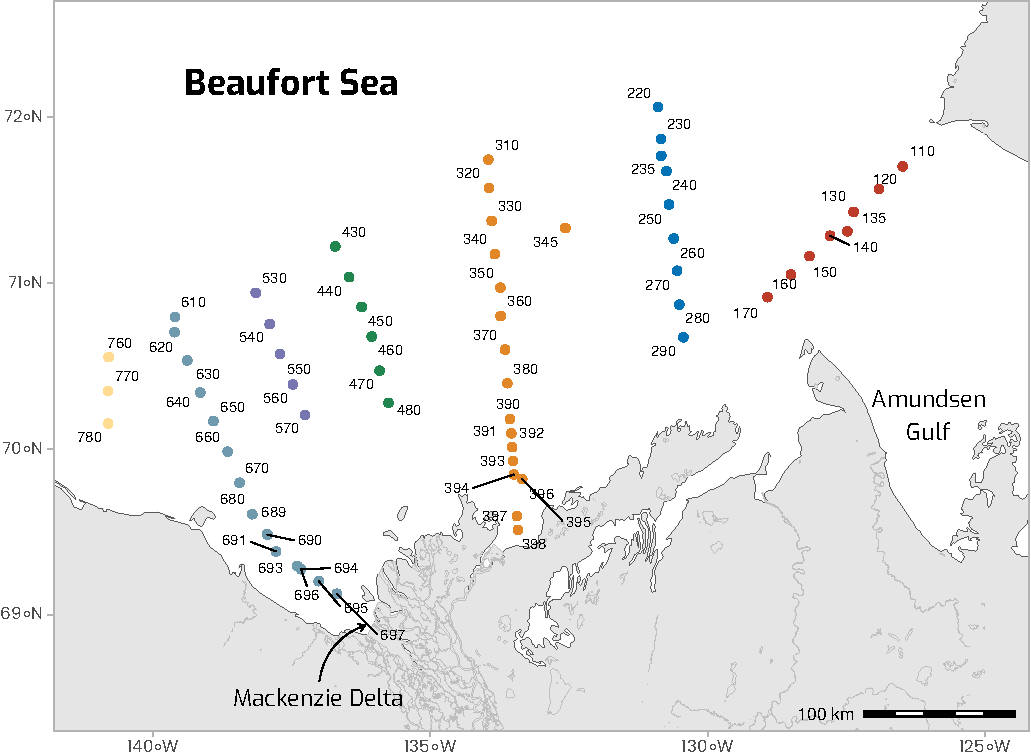
\includegraphics[scale = 1]{../../../graphs/fig01.pdf}
    \caption{(\textbf{A}) Localizations of the sampling sites visited during the MALINA 2009 campaign. The colors of the dots represent the seven transects visited during the mission. (\textbf{B}) Bathymetric profiles for transects 600 and 300. Bathymetric data from GEBCO (https://download.gebco.net/).}
\end{figure}

\clearpage

\begin{figure}[H]
    \centering
    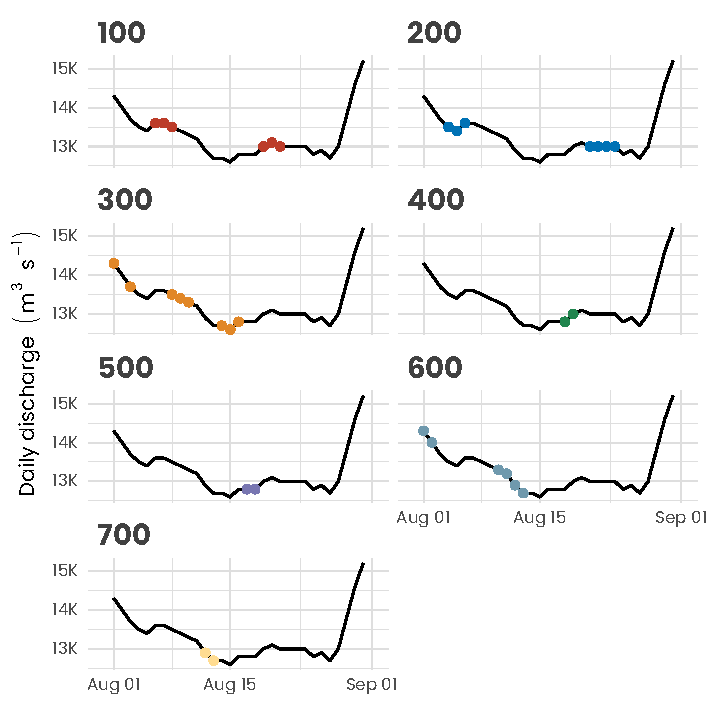
\includegraphics[scale = 1]{../../../graphs/fig02.pdf}
    \caption{(\textbf{A}) Daily discharge of the Mackenzie River at the Arctic Red River junction (station 10LC014). The black line corresponds to the 2009 discharge whereas the coloured segment identifies the period of the MALINA campaign. The shaded area is the mean discharge calculated between 1972 and 2016. Discharge data from the Government of Canada (https://wateroffice.ec.gc.ca/search/historical\_e.html). (\textbf{B}) Hourly air temperature recorded from the Amundsen's foredeck meteorological tower during the campaign.}
\end{figure}

\clearpage

\begin{figure}[H]
    \centering
    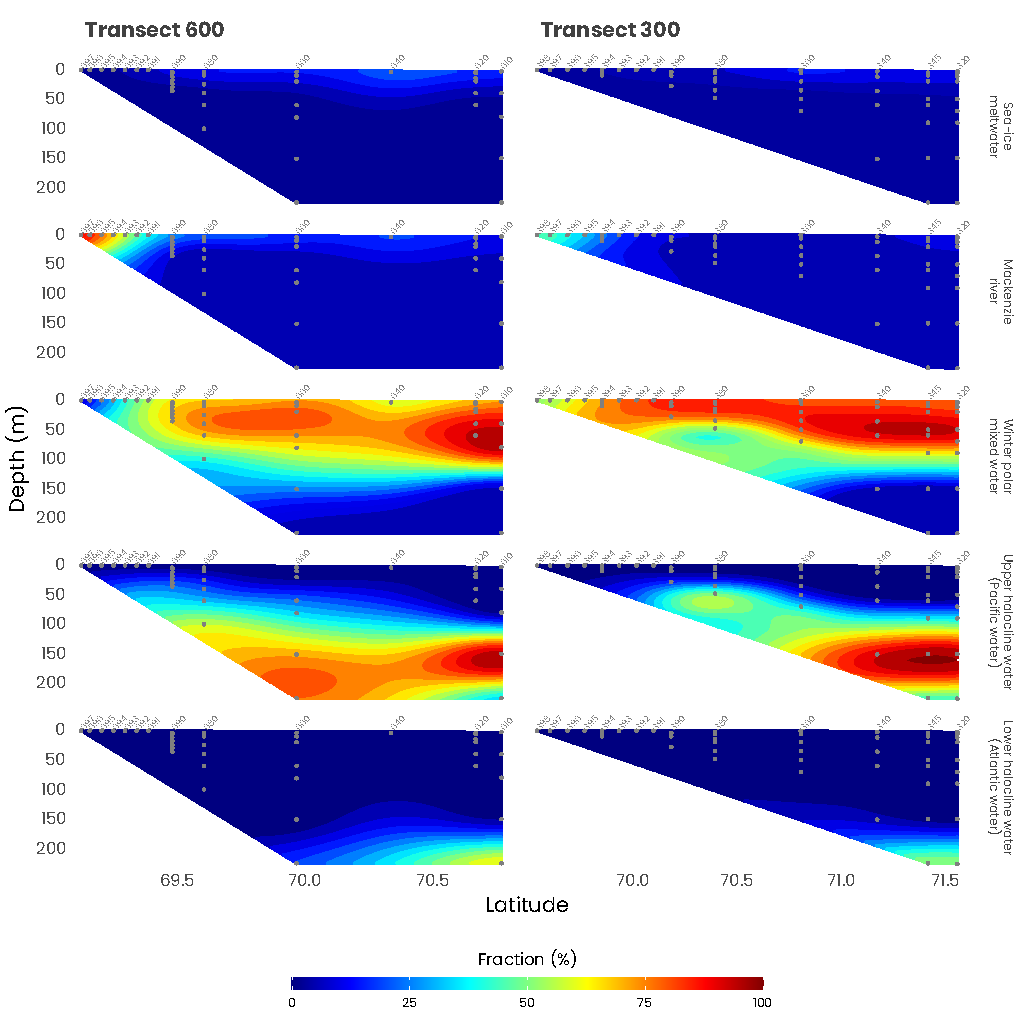
\includegraphics[scale = 1]{../../../graphs/fig03.pdf}
    \caption{Distribution of source water types along transects 600 and 300 (see Fig. 1). Station numbers are identified in light gray on top of each panel.}
\end{figure}

\clearpage

\begin{figure}[H]
    \centering
    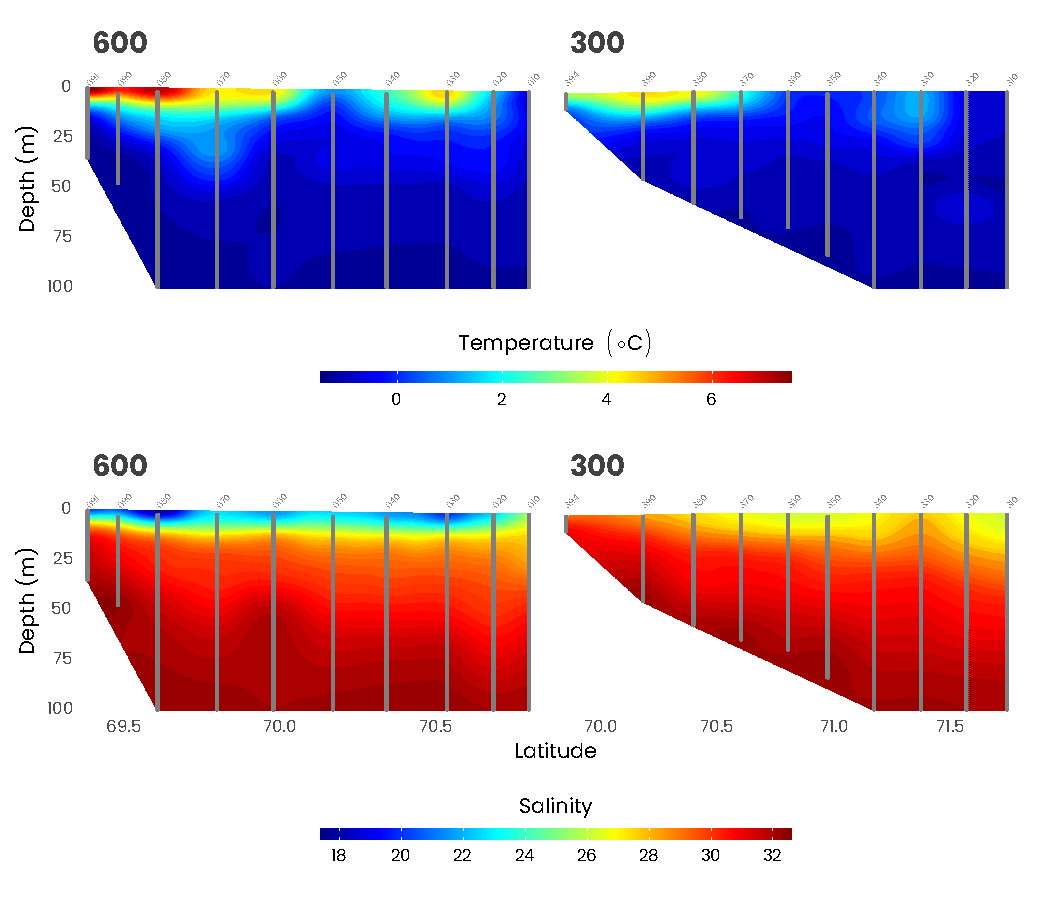
\includegraphics[scale = 1]{../../../graphs/fig04.pdf}
    \caption{Cross-sections of temperature (\textbf{A}) and salinity (\textbf{B}) measured by the CTD (gray dots) along transects 600 and 300. Station numbers are identified in light gray on top of each panel.}
\end{figure}

\clearpage

\begin{figure}[H]
    \centering
    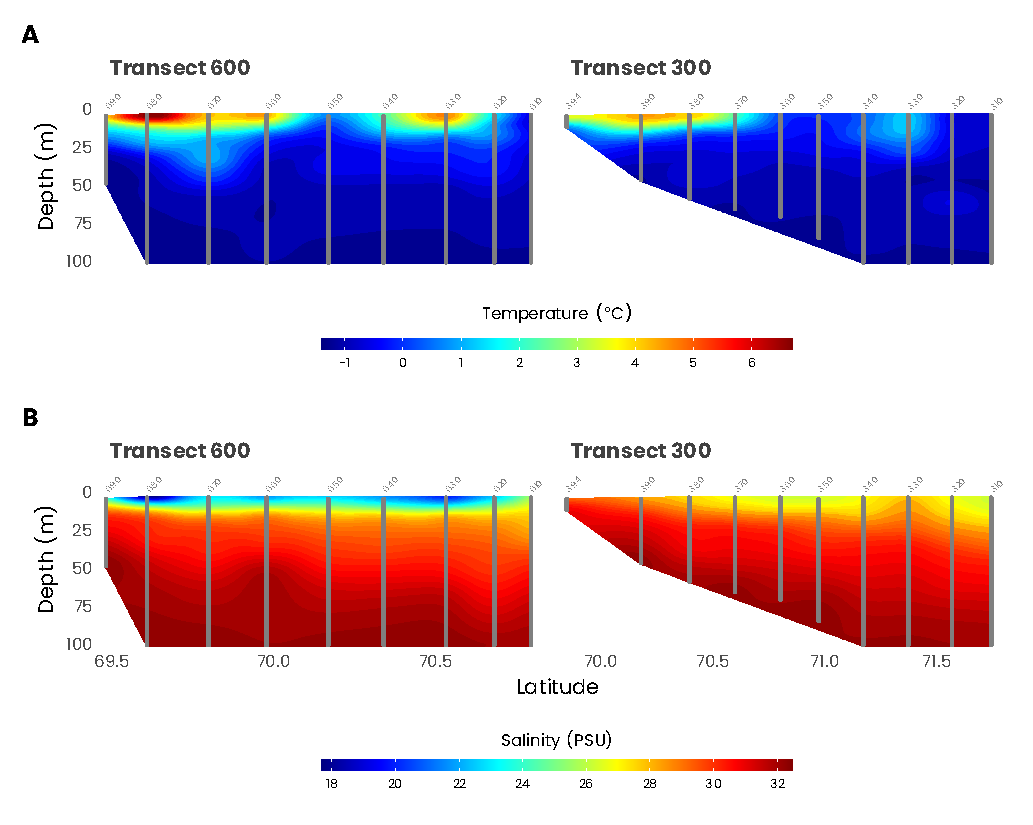
\includegraphics[scale = 0.85]{../../../graphs/fig05.pdf}
    \caption{Cross-sections of (\textbf{A}) absoprtion ($a(440)$) and (\textbf{B}) total scattering ($b_b(440)$) measured from the barge at 440 nm with an AC9 and BB9 respectively along transects 600 and 300. Station numbers are identified in light gray on top of each panel. Note that the data has been square-root transformed for the visualization.}
\end{figure}

\clearpage

\begin{figure}[H]
    \centering
    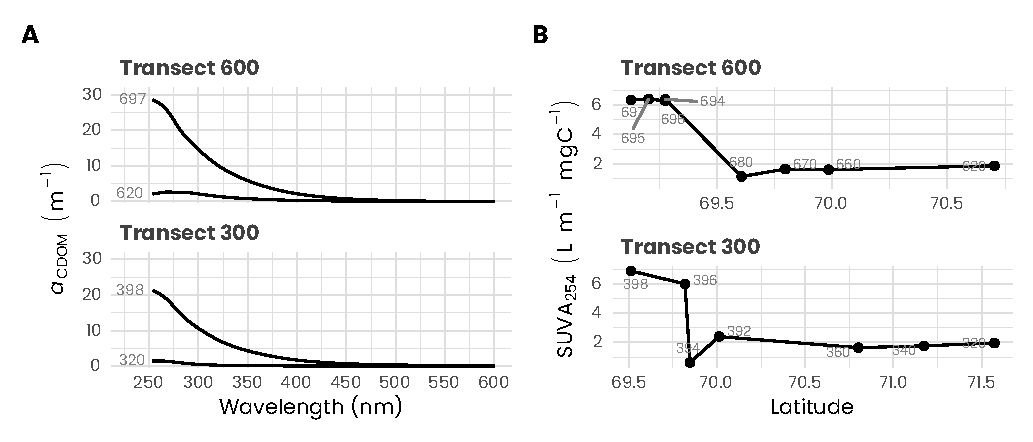
\includegraphics[scale = 1]{../../../graphs/fig06.pdf}
    \caption{(\textbf{A}) Absorption spectra between 254 and 600 nm of chromophoric dissolved organic matter ($a_{\text{CDOM}}$) measured at the surface for the northern (620, 320) and southern (697, 398) stations of the transects 600 and 300. (\textbf{B}) Particulate absorption spectra ($a_{\text{p}}$) measured between 300 and 600 nm measured at the surface for the northernmost and the southernmost stations of the transects 600 and 300. (\textbf{C}) Specific UV absorbance at 254 nm (SUVA\textsubscript{254}, i.e. absorption of light at 254 nm per unit of carbon) at surface for stations along transects 600 and 300. Stations are identified in light gray (see Fig. 1 for an overview of the station locations). Note the difference of the y-axes used in panels A and B which highlight the important differences in dissolved and particulate absorption between stations in the estuary and those offshore.}
\end{figure}

\clearpage

\begin{figure}[H]
    \centering
    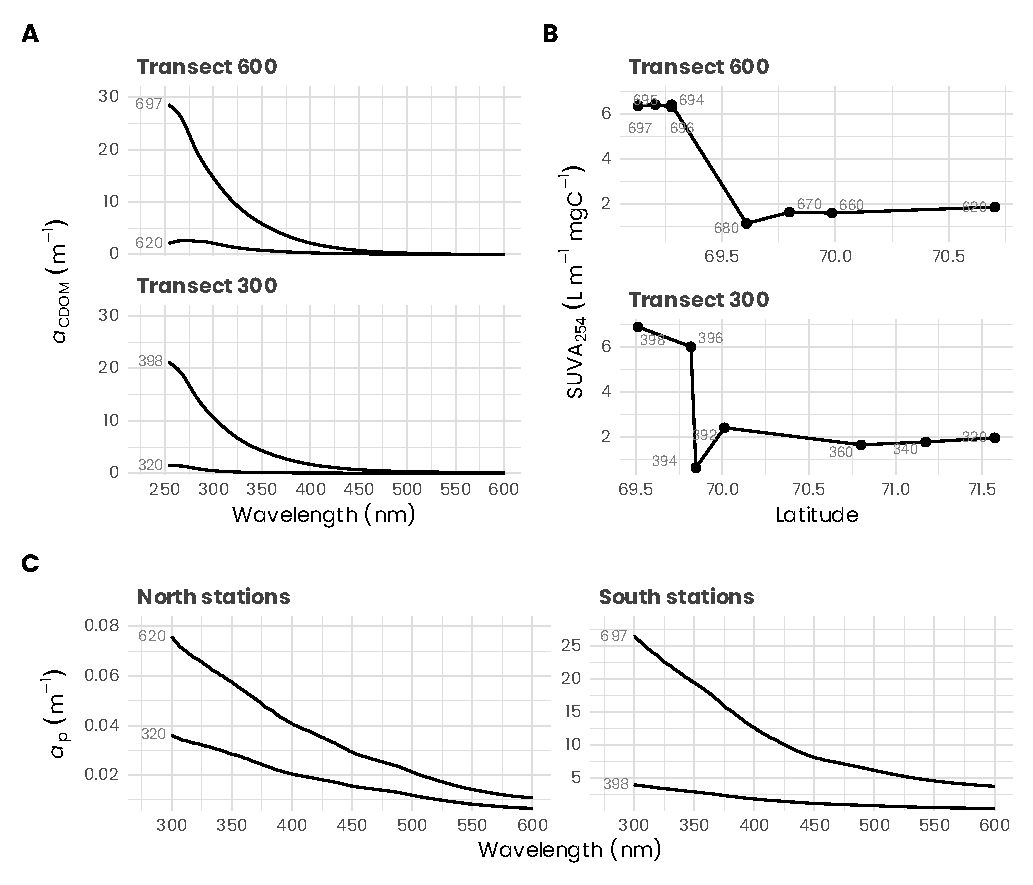
\includegraphics[scale = 0.85]{../../../graphs/fig07.pdf}
    \caption{Cross-sections of (\textbf{A}) NO$_3^-$ and (\textbf{B}) PO$_4^{3-}$ measured from Niskin bottles (gray dots) along transects 600 and 300. (\textbf{C}) N\textsuperscript{*} defined as N - rP with r = N/P = 13.1 (see the text for the details). Station numbers are identified in light gray on top of each panel.}
\end{figure}

\clearpage

\begin{figure}[H]
    \centering
    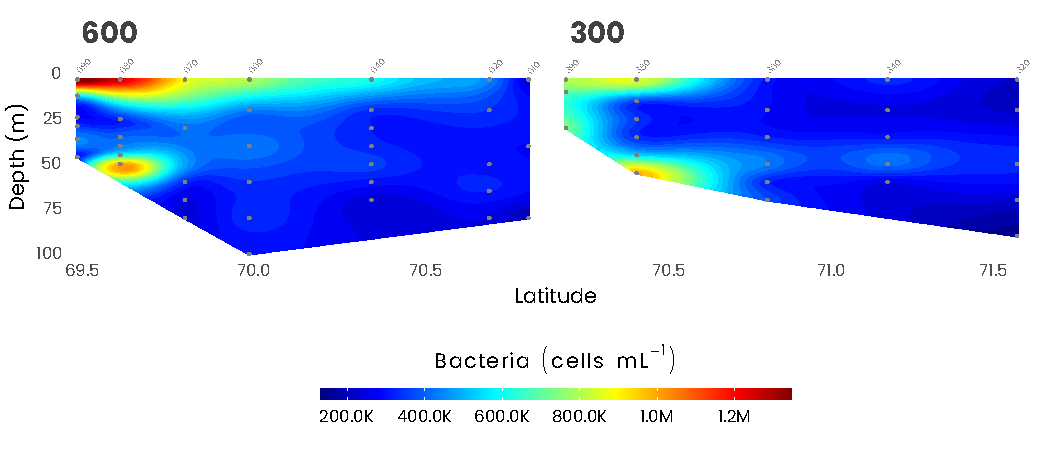
\includegraphics[scale = 1]{../../../graphs/fig08.pdf}
    \caption{Concentrations of (\textbf{A}) dissolved organic carbon (DOC), (\textbf{B}) total dissolved lignin phenols (TDLP\textsubscript{9}), and (\textbf{C}) total hydrolysable amino acids (THAA) measured along transects 600 and 300, and plotted against salinity.}
\end{figure}

\clearpage

\begin{figure}[H]
    \centering
    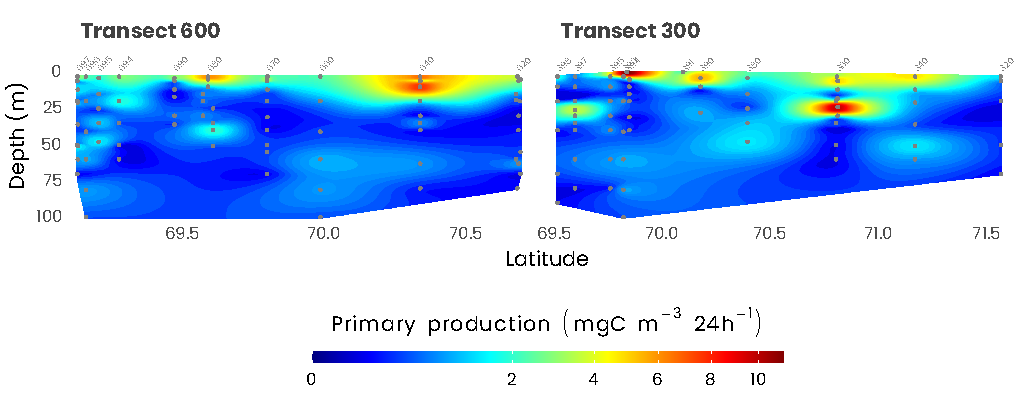
\includegraphics[scale = 1]{../../../graphs/fig09.pdf}
    \caption{Cross-sections of total chlorophyll-\textit{a} measured from HPLC (gray dots) along transects 600 and 300. Station numbers are identified in light gray on top of each panel. Note that the data has been square-root transformed for the visualization.}
\end{figure}

\clearpage

\begin{figure}[H]
    \centering
    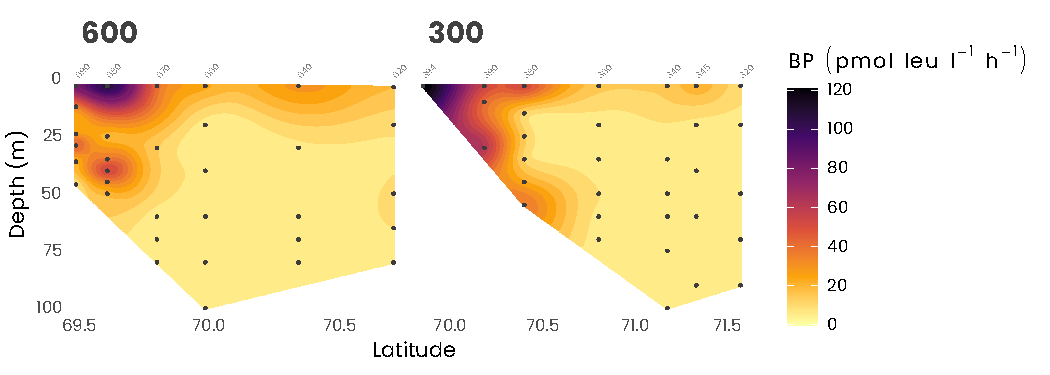
\includegraphics[scale = 1]{../../../graphs/fig10.pdf}
    \caption{Concentrations of photosynthetic (\textbf{A}) pico- and (\textbf{B}) nano-eukaryotes measured by flow cytometry during the MALINA cruise on transects 600 and 300.}
\end{figure}

\clearpage

\begin{figure}[H]
    \centering
    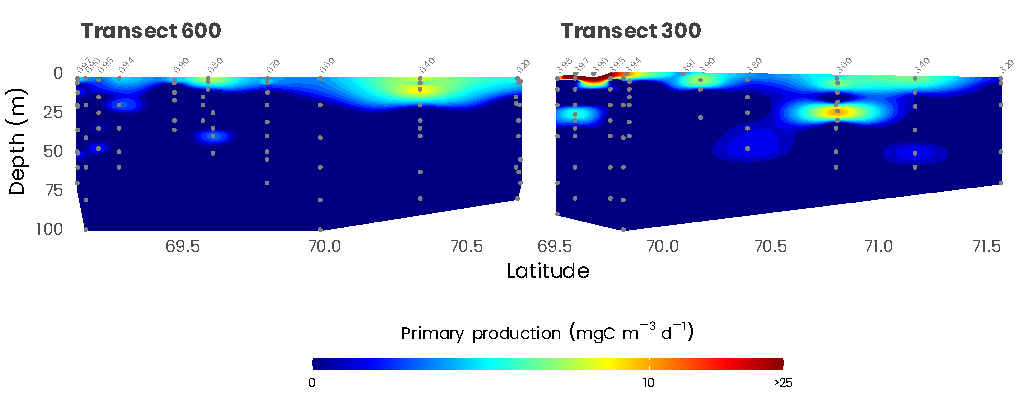
\includegraphics[scale = 1]{../../../graphs/fig11.pdf}
    \caption{(\textbf{A}) Taxonomic composition of populations of photosynthetic pico- and nano-eukaryotes sorted flow cytometry from clone library sequences  \citep{Balzano2012a}. (\textbf{B}) Taxonomic composition of cultures of phytoplankton isolated during the MALINA cruise \citep{Balzano2012b}.}
\end{figure}

\clearpage

\begin{figure}[H]
    \centering
    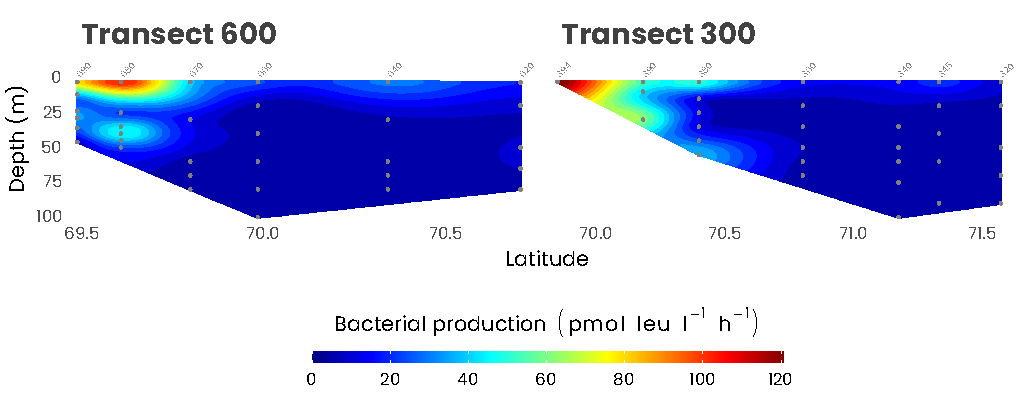
\includegraphics[scale = 1]{../../../graphs/fig12.pdf}
    \caption{Cross-sections of primary production (gray dots) along transects 600 and 300. Station numbers are identified in light gray on top of each panel. Note that the color scale is presented on a log10 scale.}
\end{figure}

\clearpage

\begin{figure}[H]
    \centering
    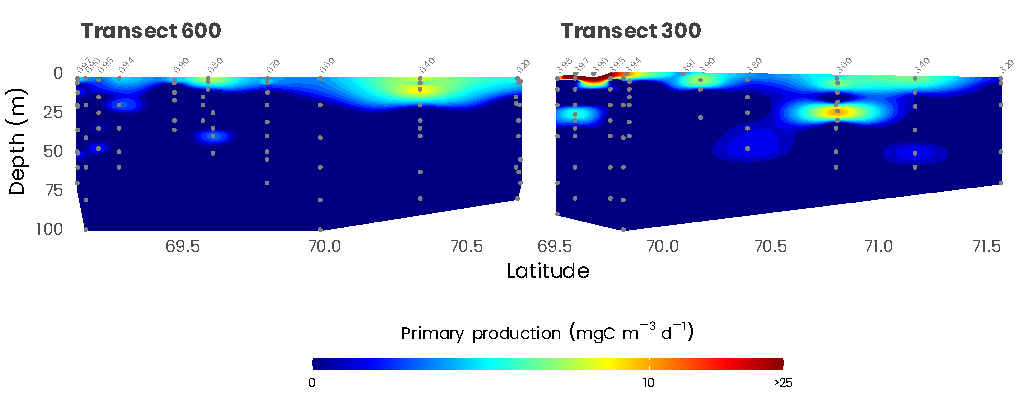
\includegraphics[scale = 1]{../../../graphs/fig13.pdf}
    \caption{(\textbf{A}) CO and CO$_2$ production measured at 295 nm at surface for stations of transects 600 and 300. (\textbf{B}) Autoxidation of suspended particulate material for stations of transects 600 and 300.}
\end{figure}

\clearpage

\begin{figure}[H]
    \centering
    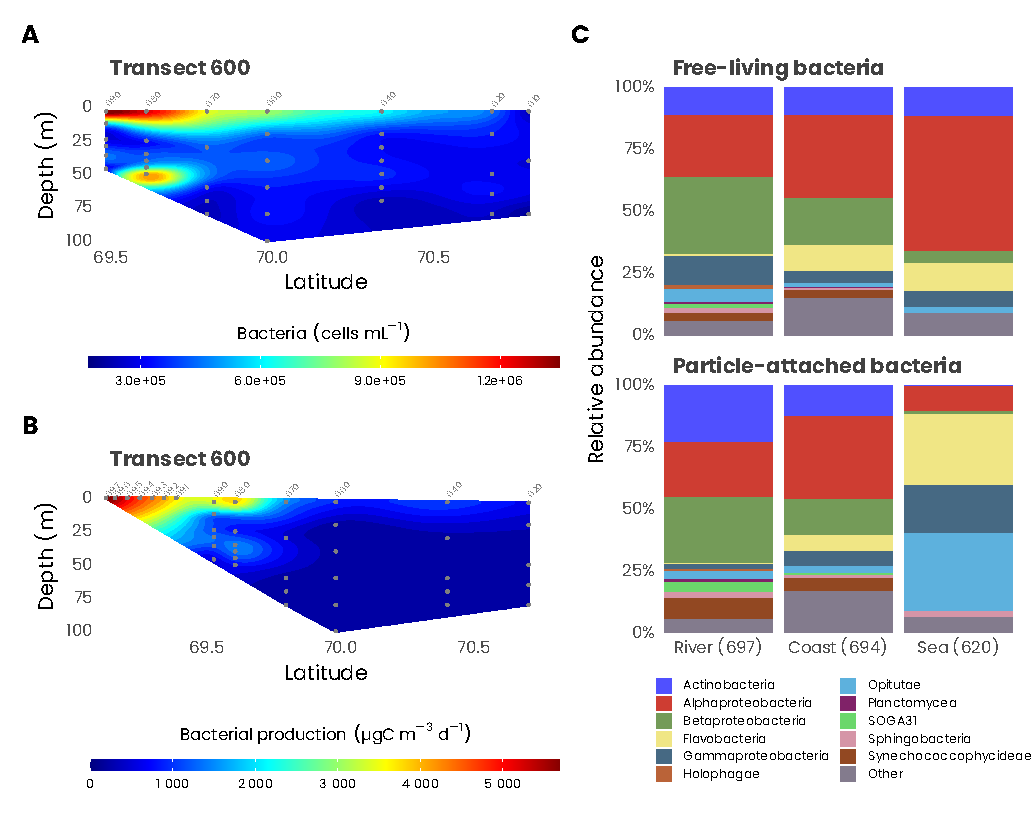
\includegraphics[scale = 1]{../../../graphs/fig14.pdf}
    \caption{(\textbf{A}) Cross-sections of bacterial abundance measured from flow cytometry and (\textbf{B}) bacterial production measured along transect 600. Station numbers are identified in light gray on top of each panel. (\textbf{C}) Cumulative bar charts comparing the relative class abundances in particle-attached (PA) and free-living (FL) for a selected number of samples in transect 600.}
\end{figure}

\clearpage

\begingroup\fontsize{5}{7}\selectfont

\begin{longtable}[t]{llll}
\caption{\label{tab:}Parameters measured during the MALINA oceanographic expedition. Parameters are ordered by alphabetical order.}\\
\toprule
Parameters & Method & Sampling & Principal investigators\\
\midrule
\endfirsthead
\caption[]{Parameters measured during the MALINA oceanographic expedition. Parameters are ordered by alphabetical order. \textit{(continued)}}\\
\toprule
Parameters & Method & Sampling & Principal investigators\\
\midrule
\endhead
\
\endfoot
\bottomrule
\endlastfoot
\textsuperscript{137}Cs datation of core samples & Gamma spectrometry & Box corer & Rochon A./ Schmidt\\
\textsuperscript{137}Cs datation of core samples & Gamma spectrometer & CASQ corer & Rochon A./ Schmidt\\
\textsuperscript{14}C datation of core samples & Accelerator Mass Spectrometry & Box corer & Rochon A.\\
\textsuperscript{14}C datation of core samples & Accelerator Mass Spectrometry & CASQ corer & Rochon A.\\
\textsuperscript{15}N-Ammonium assimilation & \textsuperscript{15}N spiking - incubation - mass-spectrometry & Rosette - Deck incubations & Tremblay J.E./ Raimbault P.\\
\addlinespace
\textsuperscript{15}N-Ammonium assimilation & \textsuperscript{15}N spiking - incubation - mass-spectrometry & Rosette In-situ production line & Tremblay J.E./ Raimbault P.\\
\textsuperscript{15}N-Ammonium oxidation (Nitrification) & \textsuperscript{15}N spiking - incubation - mass-spectrometry & Rosette - Deck incubations & Tremblay J.E./ Raimbault P.\\
\textsuperscript{15}N-Ammonium oxidation (Nitrification) & \textsuperscript{15}N spiking - incubation - mass-spectrometry & Rosette In-situ production line & Tremblay J.E./ Raimbault P.\\
\textsuperscript{15}N-Ammonium primary production (\textsuperscript{13}C) & \textsuperscript{15}N spiking - incubation - mass-spectrometry & Rosette - Deck incubations & Tremblay J.E./ Raimbault P.\\
\textsuperscript{15}N-Ammonium regeneration & \textsuperscript{15}N spiking - incubation - mass-spectrometry & Rosette - Deck incubations & Tremblay J.E./ Raimbault P.\\
\addlinespace
\textsuperscript{15}N-Ammonium regeneration & \textsuperscript{15}N spiking - incubation - mass-spectrometry & Rosette In-situ production line & Tremblay J.E./ Raimbault P.\\
\textsuperscript{15}N-N\textsubscript{2} fixation & \textsuperscript{15}N spiking - incubation - mass-spectrometry & Rosette water sample & Tremblay J.E./ Raimbault P.\\
\textsuperscript{15}N-Nitrate assimilation & \textsuperscript{15}N spiking - incubation - mass-spectrometry & Rosette - Deck incubations & Tremblay J.E./ Raimbault P.\\
\textsuperscript{15}N-Nitrate assimilation & \textsuperscript{15}N spiking - incubation - mass-spectrometry & Rosette In-situ production line & Tremblay J.E./ Raimbault P.\\
\textsuperscript{15}N-Urea Photosynthetic parameters & \textsuperscript{15}N incubations mass spectrometry & Rosette Niskin water sample & Tremblay J.E.\\
\addlinespace
\textsuperscript{210}Pb geochronology of core samples & \textsuperscript{209}Po alpha spectrometry & Box corer & Rochon A.\\
\textsuperscript{210}Pb geochronology of core samples & \textsuperscript{209}Po alpha spectrometry & CASQ corer & Rochon A.\\
\textsuperscript{226}Ra (particulate) & Gamma spectrometry & Foredeck In-situ pump & Gasser B.\\
\textsuperscript{226}Ra/228Ra & Gamma spectrometry & Discrete Sample on Continuous System. & Gasser B.\\
\textsuperscript{234}Th (1 micron < particles > 70 micron) & Beta-counting & Foredeck In-situ pump & Gasser B.\\
\addlinespace
\textsuperscript{234}Th (particles > 70 micron) & Beta-counting & Foredeck In-situ pump & Gasser B.\\
\textsuperscript{234}Th (Particulate) & Beta-counting & Drifting Sediment trap & Gasser B.\\
\textsuperscript{234}Th (total) & Beta-counting & Rosette water sample & Gasser B.\\
\textsuperscript{238}U (Dissolved) & Derived parameter & Rosette water sample & Gasser B.\\
\textsuperscript{238}U (total) & Alpha-counting & Rosette water sample & Gasser B.\\
\addlinespace
AAPB (abundance) & IR microscopy, fluorimetry. FISH & Rosette water sample & Jeanthon C./ Boeuf D.\\
AAPB (abundance) & IR microscopy, fluorimetry. FISH & Zodiac water sample & Jeanthon C./ Boeuf D.\\
Absorption (particulate) & PSICAM & Barge water sample & Leymarie E.\\
Absorption (particulate) & Spectrophotometer (filters) & Barge water sample & Belanger S.\\
Absorption (particulate) & Spectrophotometer (filters) & Continuous on way & Belanger S.\\
\addlinespace
Absorption (particulate) & PSICAM & Rosette water sample & Leymarie E.\\
Absorption (particulate) & Spectrophotometer (filters) & Rosette water sample & Belanger S.\\
Absorption (particulate) & Spectrophotometer (filters) & Zodiac profiler & Belanger S.\\
Absorption (total) & PSICAM & Barge water sample & Leymarie E.\\
Absorption (total) & PSICAM & Rosette water sample & Leymarie E.\\
\addlinespace
Absorption coefficient (total) & HOBI-Labs a-sphere & Barge profiler & Wright V./ Hooker S.\\
Absorption coefficient (total) (9 wavelengths) & Wetlabs AC9 Serial\# 156 & Rosette profiler & Ehn J.\\
Absorption coefficient (total) (9 wavelengths in IR & Wetlabs AC9 Serial\# 303 & Barge profiler & Doxaran D.\\
Absorption coefficient (total) (9 wavelengths) & Wetlabs AC9 Serial\# 279 & Barge profiler & Doxaran D.\\
Air Relative Humidity & Humidity Sensor & Foredeck Meteorological Tower & Papakyriakou T.\\
\addlinespace
Alkalinity total (TA) & Potentiometry & Barge water sample & Mucci A./ Lansard B.\\
Alkalinity total (TA) & Potentiometry & Rosette & Mucci A./ Lansard B.\\
Alkalinity total (TA) & Potentiometry & Zodiac water sample & Mucci A./ Lansard B.\\
Alkanes & GC-MS & Box corer & Bouloubassi I.\\
Alkanes & GC-MS & CASQ corer & Bouloubassi I.\\
\addlinespace
Ammonium (NH$^+_4$) photo-production apparent quantum yield (AQY) & sun simulator - fluorimetry & Rosette water sample & Xie H./ Tremblay J.E.\\
Ammonium (NH$^+_4$) photo-production apparent quantum yield (AQY) & sun simulator - fluorimetry & Zodiac water sample & Xie H./ Tremblay J.E.\\
Aragonite : saturation state & Derived parameter & Barge water sample & Mucci A./ Lansard B.\\
Aragonite : saturation state & Derived parameter & Rosette water sample & Mucci A./ Lansard B.\\
Aragonite : saturation state & Derived parameter & Zodiac water sample & Mucci A./ Lansard B.\\
\addlinespace
Archaea (diversity) & CE-SSCP and DNA clone library & Rosette water sample & Joux F.\\
Attenuation coefficient (total) (9 wavelengths in IR) & Wetlabs AC9 Serial \#0303 & Barge profiler & Doxaran D.\\
Attenuation coefficient (total) (9 wavelengths) & Wetlabs AC9 Serial \#279 & Barge profiler & Doxaran D.\\
Attenuation coefficient (total) (9 wavelengths) & Wetlabs AC9 Serial \#156 & Rosette profiler & Ehn J.\\
Attenuation coefficient at 660 nm & Wetlabs (CRover) transmissometer & Drifting profiling float & Doxaran D.\\
\addlinespace
Backscattering 532 nm & Wetlabs (ECO3) backscatterometer & Drifting profiling float & Doxaran D.\\
Backscattering coefficient (3 wavelengths in IR) & Wetlabs ECO-BB3 serial \#538 & Barge profiler & Doxaran D.\\
Backscattering coefficient (3 wavelengths) & Wetlabs ECO-BB3 serial \#028 & Barge profiler & Doxaran D.\\
Backscattering coefficient (6 Wavelength) & HOBI-Labs Hydroscat-6 serial \# & Barge profiler & Wright V./ Hooker S.\\
Backscattering coefficient (8 wavelengths, spectral) & Hydroscat-6 (ser\#97074) and two a-Beta (HOBI-Labs) & Barge profiler & Reynolds R.\\
\addlinespace
Backscattering coefficient (8 wavelengths, spectral) & Hydroscat-6 (ser\#97074) and two a-Beta (HOBI-Labs) & Foredeck & Reynolds R.\\
Backscattering coefficient (9 wavelengths) & Wetlabs ECO-BB9 serial\# 274 & Rosette profiler & Ehn J.\\
Bacteria (abundance) & Flow cytometry & Rosette water sample & Vaulot D.\\
Bacteria (abundance) & Flow Cytometry & Rosette water sample & Joux F./ Ortega E.\\
Bacterial abundance & FISH-TSA & Rosette water sample & Joux F.\\
\addlinespace
Bacterial bio-volume & Epifluorescence microscopy & Rosette water sample & Joux F./ Ortega E.\\
Bacterial density (benthic) & Flow cytometry & Box corer & Link H./ Archambault P./ Chaillou G.\\
Bacterial diversity & CE-SSCP and DNA clone library & Rosette water sample & Joux F.\\
Bacterial Ecto-enzymatic activity & Spectrofluorimetry & Rosette water sample & Joux F./ Ortega E.\\
Bacterial growth (limitation by nutrients) & Leu-3H incubations - cells counts & Rosette water sample & Joux F./ Jeffrey W./ Ortega E.\\
\addlinespace
Bacterial production & Leucine-3H incorporation & Rosette water sample & Joux F./ Jeffrey W.\\
Bacterial production & Leucine-3H incorporation & Zodiac water sample & Joux F./ Jeffrey W.\\
Bacterial production (effects of DOM UV exposure on...) & Leucine-3H incorporation - cell counts & Rosette water sample & Joux F./ Jeffrey W./ Ortega E.\\
Bacterial production (effects of UV radiation) & Leucine-3H incorporation & Rosette water sample & Joux F./ Jeffrey W.\\
Bacterial respiration (whole community) & O\textsuperscript{2} consumption - Winkler - Incubations & Rosette water sample & Joux F./ Ortega E.\\
\addlinespace
Benthic ammonium flux & Incubations - Colorimetry & Box corer & Link H./ Archambault P./ Chaillou G.\\
Benthic DOC remineralisation & Incubations - wet oxidation & Box corer & Link H./ Archambault P./ Chaillou G./ Charriere B.\\
Benthic Macrofauna abundance & Microscopy & Box corer & Link H./ Archambault P./ Chaillou G.\\
Benthic Macrofauna biomass & Wet weight & Box corer & Link H./ Archambault P./ Chaillou G.\\
Benthic Macrofauna diversity & Microscopy & Box corer & Link H./ Archambault P./ Chaillou G.\\
\addlinespace
Benthic nitrate flux & Incubations - Colorimetry- Autoanalyzer & Box corer & Link H./ Archambault P./ Chaillou G.\\
Benthic nitrite flux & Incubations - Colorimetry- Autoanalyzer & Box corer & Link H./ Archambault P./ Chaillou G.\\
Benthic phosphate flux & Incubations - Colorimetry- Autoanalyzer & Box corer & Link H./ Archambault P./ Chaillou G.\\
Benthic respiration & Incubations - Optic - Oxygen probe & Box corer & Link H./ Archambault P./ Chaillou G.\\
Benthic silicic acid flux & Incubations - Colorimetry - Autoanalyzer & Box corer & Link H./ Archambault P./ Chaillou G.\\
\addlinespace
Bioturbation of sediments & Incubation with luminophores & Box corer & Link H./ Archambault P./ Chaillou G.\\
Calcite : saturation state & Derived parameter & Barge water sample & Mucci A./ Lansard B.\\
Calcite : saturation state & derived parameter & Rosette water sample & Mucci A./ Lansard B.\\
Calcite : saturation state & Derived parameter & Zodiac water sample & Mucci A./ Lansard B.\\
Campesterol, cholesterol, sistosterol and products of degrad & GC-MS & Rosette water sample & Sempere R.\\
\addlinespace
CDOM absorption & PSICAM & Barge water sample & Leymarie E.\\
CDOM absorption & Spectrophotometer & Barge water sample & Matsuoka A./ Bricaud A.\\
CDOM absorption & Spectrophotometer & Barge water sample & Wright V./ Hooker S.\\
CDOM absorption & Ultrapath & Barge water sample & Bricaud A.\\
CDOM absorption & PSICAM & Rosette water sample & Leymarie E.\\
\addlinespace
CDOM absorption & Spectrophotometer & Rosette water sample & Matsuoka A./ Bricaud A.\\
CDOM absorption & Ultrapath & Rosette water sample & Bricaud A.\\
CDOM absorption & PSICAM & Zodiac water sample & Leymarie E.\\
CDOM absorption & Spectrophotometer & Zodiac water sample & Matsuoka A./ Bricaud A.\\
CDOM absorption & Ultrapath & Zodiac water sample & Bricaud A.\\
\addlinespace
CDOM fluorescence & HOBI-Labs Hydroscat-6 ser\# HS080542 & Barge profiler & Wright V./ Hooker S.\\
CDOM fluorescence & Wetlabs WetStar WSCD & Barge profiler & Doxaran D.\\
CDOM fluorescence & Wetlabs (ECO3) fluorometer & Drifting profiling float & Doxaran D.\\
CDOM fluorescence & Haardt fluorometer & Rosette profiler & Belanger S./ Amon/ Sempere R.\\
CDOM fluorescence EEM (excitation-emission-matrix) & Spectrofluorimetry & Rosette water sample & Belanger S./ Amon/ Sempere R.\\
\addlinespace
CDOM fluorescence EEM (excitation-emission-matrix) & Spectrofluorimetry & Zodiac water sample & Belanger S./ Amon/ Sempere R.\\
Chlorophyll a and Phaeopigments (concentration) & Fluorimetry Size fractionned & Rosette water sample & Gosselin M./ Belanger S.\\
Chlorophyll a and Phaeopigments (benthic) & Fluorometric analysis & Box corer & Link H./ Archambault P./ Chaillou G.\\
Chlorophyll a fluorescence [Fchla (z)] & Chelsea Mini-Track a II fluorometer & Barge profiler & Doxaran D.\\
Chlorophyll a fluorescence [Fchla (z)] & HOBI-Labs Hydroscat-6 fluorometer & Barge profiler & Wright V./ Hooker S.\\
\addlinespace
Chlorophyll a fluorescence [Fchla (z)] & Wetlabs (ECO3) fluorometer & Drifting profiling float & Doxaran D.\\
Chlorophyll a fluorescence [Fchla (z)] & SeaPoint fluorometer & Rosette profiler & Gratton Y./ Prieur L./ Tremblay J.E.\\
CO photo-prod. apparent quantum yield for CDOM & Sun simulator - reduction gas analyzer & Rosette water sample & Xie H.\\
CO photo-prod. apparent quantum yield for CDOM & Sun simulator - reduction gas analyzer & Zodiac water sample & Xie H.\\
CO photo-prod. apparent quantum yield for particulate matter & Sun simulator - reduction gas analyzer & Rosette water sample & Xie H.\\
\addlinespace
CO photo-prod. apparent quantum yield for particulate matter & Sun simulator - reduction gas analyzer & Zodiac water sample & Xie H.\\
CO\textsuperscript{2} (atm) concentration & Infra Red & Foredeck Meteorological Tower & Papakyriakou T.\\
CO\textsuperscript{2} (seawater) concentration & Infra Red & Foredeck Meteorological Tower & Papakyriakou T.\\
CO3 2- concentrations & Derived parameter & Barge water sample & Mucci A./ Lansard B.\\
CO3 2- concentrations & Derived parameter & Rosette water sample & Mucci A./ Lansard B.\\
\addlinespace
CO3 2- concentrations & Derived parameter & Zodiac water sample & Mucci A./ Lansard B.\\
Coccolithophorids & Microscopy & Rosette water sample & Coupel P.\\
Conductivity (z) & Sensor on SBE Fascat CTD serial \# & Barge profiler & Doxaran D.\\
Conductivity (z) & Sensor on SBE Fascat CTD serial \# & Barge profiler & Wright V./ Hooker S.\\
Conductivity (z) & Sensor SeaBird 4c on CTD SBE-911 & Rosette profiler & Gratton Y./ Prieur L.\\
\addlinespace
CTD & Seabird & Drifting profiling float & Doxaran D.\\
Cultures of sorted populations & Sorted by flow cytometry, serial dilution and single cell pipetting & Rosette water sample & Vaulot D.\\
Current Profile [U (z)] & ADCP (LADCP) RD Instrument 300 KHz & Rosette profiler & Marec C./ Gratton Y./ Prieur L.\\
delta \textsuperscript{13}C & Mass Spectrometry & Zodiac water sample & Mucci A./ Lansard B.\\
delta \textsuperscript{13}C on suspended particulate matter & Mass Spectrometry & Rosette water sample & Tremblay J.E./ Raimbault P.\\
\addlinespace
delta \textsuperscript{15}C on suspended particulate matter & Mass Spectrometry & Rosette water sample & Tremblay J.E./ Raimbault P.\\
delta \textsuperscript{18}O - water & Mass Spectrometry & Rosette water sample & Mucci A./ Lansard B.\\
delta \textsuperscript{18}O - water & Mass Spectrometry & Zodiac water sample & Mucci A./ Lansard B.\\
delta\textsuperscript{13}C & Mass Spectrometer & Barge water sample & Mucci A./ Lansard B.\\
delta\textsuperscript{13}C & Mass Spectrometry & Rosette water sample & Mucci A./ Lansard B.\\
\addlinespace
delta\textsuperscript{18}O - water & Mass Spectrometry & Barge water sample & Mucci A./ Lansard B.\\
Diacids composition & GC/MS & Rosette water sample & Sempere R.\\
Diacids composition & GC/MS & Zodiac water sample & Sempere R.\\
Diacids photo-production apparent quantum yield (AQY) & Sun simulator - GC/MS & Zodiac water sample & Sempere R.\\
Dinoflagellates cysts Abundance & Microscopy & Box corer & Rochon A.\\
\addlinespace
Dinoflagellates cysts Abundance & Microscopy & CASQ corer & Rochon A.\\
Dinoflagellates cysts Identification & Microscopy & Box corer & Rochon A.\\
Dinoflagellates cysts Identification & Microscopy & CASQ corer & Rochon A.\\
Dissolved Inorg. Carbon photo-prod. apparent quantum yield & Sun simulator - indrared CO\textsuperscript{2} analyzer & Rosette water sample & Xie H./ Belanger S.\\
Dissolved Inorg. Carbon photo-prod. apparent quantum yield & Sun simulator - indrared CO\textsuperscript{2} analyzer & Zodiac water sample & Xie H./ Belanger S.\\
\addlinespace
Dissolved Organic Carbon (DOC) & High Temperature Catalytic Oxidation & Barge water sample & Wright V./ Hooker S.\\
Dissolved Organic Carbon (DOC) & High Temperature Catalytic Oxidation & Rosette water sample & Sempere R.\\
Dissolved Organic Carbon (DOC) & High Temperature Catalytic Oxidation & Rosette water sample & Benner R.\\
Dissolved Organic Carbon (DOC) & Wet oxidation & Rosette water sample & Tremblay J.E./ Raimbault P.\\
Dissolved Organic Carbon (DOC) & High Temperature Catalytic Oxidation & Zodiac water sample & Sempere R.\\
\addlinespace
Dissolved Organic Carbon (DOC) & High Temperature Catalytic Oxidation & Zodiac water sample & Benner R.\\
Dissolved Organic Nitrogen (DON) & Wet oxidation & Rosette water sample & Tremblay J.E./ Raimbault P.\\
Dissolved Organic Nitrogen (Total) (TDON) & High Temperature Catalytic Oxidation & Rosette water sample & Benner R.\\
Dissolved Organic Nitrogen (Total) (TDON) & High Temperature Catalytic Oxidation & Zodiac water sample & Benner R.\\
Dissolved Organic Phosphorus (DOP) & Wet oxidation & Rosette water sample & Tremblay J.E./ Raimbault P.\\
\addlinespace
Ed, Lu, Eu, Es & C-OPS package (320, 340, 380, 395 nm) & Barge profiler & Hooker\\
Electric resistivity (sediment core physical properties) & Geotek Multi Sensor Core Logger & Box corer & Rochon A.\\
Electric resistivity (sediment core physical properties) & Geotek Multi Sensor Core Logger & CASQ corer & Rochon A.\\
Eukaryotes (abundance) & DAPI epifluorescence microscopy & Rosette water sample & Lovejoy C.\\
Eukaryotes (abundance) & FISH-TSA & Rosette water sample & Lovejoy C.\\
\addlinespace
Eukaryotes (biomass) & DAPI epifluorescence microscopy & Rosette water sample & Lovejoy C.\\
fCO\textsuperscript{2} & Derived parameter & Barge water sample & Mucci A./ Lansard B.\\
fCO\textsuperscript{2} & Derived parameter & Rosette water sample & Mucci A./ Lansard B.\\
fCO\textsuperscript{2} & Derived parameter & Zodiac water sample & Mucci A./ Lansard B.\\
Foraminifera abundance & Microscopy & Box corer & Rochon A.\\
\addlinespace
Foraminifera abundance & Microscopy & CASQ corer & Rochon A.\\
Foraminifera identification & Microscopy & Box corer & Rochon A.\\
Foraminifera identification & Microscopy & CASQ corer & Rochon A.\\
Gamma density (sediment core physical properties) & Geotek Multi Sensor Core Logger & Box corer & Rochon A.\\
Gamma density (sediment core physical properties) & Geotek Multi Sensor Core Logger & CASQ corer & Rochon A.\\
\addlinespace
H\textsubscript{2}O (atm) concentration & Infrared gas analyzer & Foredeck Meteorological Tower & Papakyriakou T.\\
HCO\textsuperscript{2}- concentration & Derived parameter & Barge water sample & Mucci A./ Lansard B.\\
HCO\textsuperscript{2}- concentration & Derived parameter & Rosette water sample & Mucci A./ Lansard B.\\
HCO\textsuperscript{2}- concentration & Derived parameter & Zodiac water sample & Mucci A./ Lansard B.\\
Hydro SCAMP (Temp, Salin, Chlorophyll, turb. ...) & SCAMP profiler & In-water profiler & Gratton Y.\\
\addlinespace
Hydrolysable Amino Acids (Total) (THAA) & HPLC & Rosette water sample & Benner R.\\
Hydrolysable Amino Acids (Total) (THAA) & HPLC & Zodiac water sample & Benner R.\\
Hydroxyl radicals (OH) & HPLC & Rosette water sample & Sempere R.\\
Hydroxyl radicals (OH) & HPLC & Zodiac water sample & Sempere R.\\
Hydroxyl radicals (OH) photo-prod. apparent quantum yield & Sun simulator - HPLC & Rosette water sample & Sempere R.\\
\addlinespace
Hydroxyl radicals (OH) photo-prod. apparent quantum yield & Sun simulator - HPLC & Zodiac water sample & Sempere R.\\
IP25 (C25 Monounsaturated Hydrocarbon) & GC & Box corer & Masse G.\\
IP25 (C25 Monounsaturated Hydrocarbon) & GC & CASQ corer & Masse G.\\
Irradiance & Satlantic (PUV) (305,325, 340, 380,..) & Foredeck & Sempere R.\\
Irradiance (412, 490, 555 nm) & Satlantic (OCR) radiometer & Drifting profiling float & Doxaran D.\\
\addlinespace
Lignin phenols (dissolved) & GC/MS & Rosette water sample & Benner R.\\
Lignin phenols (dissolved) & GC/MS & Zodiac water sample & Benner R.\\
Lipid biomarqueurs & GC-Flamme Ionization Detection / GC-MS & Box corer & Tolosa I.\\
Lipid biomarqueurs & GC-Flamme Ionization Detection / GC-MS & CASQ corer & Tolosa I.\\
Lipid biomarqueurs d\textsuperscript{13}C & GC-Combustion Isotope ratio MS & Box corer & Tolosa I.\\
\addlinespace
Lipid biomarqueurs d\textsuperscript{13}C & GC-Combustion Isotope ratio MS & CASQ corer & Tolosa I.\\
Long-Wave radiation (Lwin) & Pyrgeometer & Wheel-house radiation platform & Papakyriakou T.\\
Magnetic susceptibility (sediment core physical properties) & Geotek Multi Sensor Core Logger & Box corer & Rochon A.\\
Magnetic susceptibility (sediment core physical properties) & Geotek Multi Sensor Core Logger & CASQ corer & Rochon A.\\
Nanoeukaryotes (abundance) & Flow cytometry & Rosette water sample & Vaulot D.\\
\addlinespace
NH$^+_4$ & Fluorescence & Rosette water sample & Tremblay J.E./ Raimbault P.\\
Nitrate (concentration) & Satlantic ISUS & Rosette profiler & Gratton Y./ Prieur L./ Tremblay J.E.\\
NO$^-_2$ & Colorimetry/Autoanalyzer & Rosette water sample & Tremblay J.E./ Raimbault P.\\
NO$^-_3$ & Colorimetry/Autoanalyzer & Rosette water sample & Tremblay J.E./ Raimbault P.\\
Organic Compounds High Molecular Weight (HMW) & Sun simulator incubations - HPLC & Rosette water sample & Xie H.\\
\addlinespace
Organic Compounds High Molecular Weight (HMW) & Sun simulator incubations - HPLC & Zodiac water sample & Xie H.\\
Organic Compounds Low Molecular Weight (LMW) & Sun simulator incubations - HPLC & Rosette water sample & Xie H.\\
Organic Compounds Low Molecular Weight (LMW) & Sun simulator incubations - HPLC & Zodiac water sample & Xie H.\\
Oxygen (dissolved) & Discrete samples Winkler Method & Barge water sample & Prieur L.\\
Oxygen (dissolved) & Idronaut Ocean Seven O\textsuperscript{2} sensor & Continuous horizontal & Papakyriakou T.\\
\addlinespace
Oxygen (dissolved) & SeaBird SBE-43 sensor & Rosette profiler & Gratton Y./ Prieur L.\\
Oxygen (dissolved) & Discrete samples Winkler Method & Rosette water sample & Prieur L.\\
Oxygen (dissolved) & Discrete samples Winkler Method & Zodiac water sample & Prieur L.\\
P waves speed (sediment core physical properties) & Geotek Multi Sensor Core Logger & Box corer & Rochon A.\\
P waves speed (sediment core physical properties) & Geotek Multi Sensor Core Logger & CASQ corer & Rochon A.\\
\addlinespace
Paleomagnetism & Cryogenic magnetometer & Box corer & Rochon A.\\
Paleomagnetism & Cryogenic magnetometer & CASQ corer & Rochon A.\\
PAR & Biospherical sensor & Barge profiler & Wright V./ Hooker S.\\
PAR & Biospherical sensor & Rosette profiler & Gratton Y./ Prieur L./ Tremblay J.E.\\
PAR & PARLite sensor & Wheel-house radiation platform & Papakyriakou T.\\
\addlinespace
Particle Size Distribution & LISST-100X & Barge profiler & Reynolds R.\\
Particle Size Distribution & Coulter counter & Barge water sample & Reynolds R.\\
Particle Size Distribution & UVP-5 & In-water profiler & Picheral M.\\
Particle Size Distribution & LISST-100X & Rosette profiler & Reynolds R.\\
Particle Size Ditribution & Coulter counter & Rosette water sample & Reynolds R.\\
\addlinespace
Particulate Organic Carbon (POC) & CHN analyzer & Barge water sample & Wright V./ Hooker S.\\
Particulate Organic Carbon (POC) & CHN analyzer on SPM filters & Barge water sample & Doxaran D./ Ehn J./ Babin M.\\
Particulate Organic Carbon (POC) & CHN analyzer on SPM filters & Rosette water sample & Doxaran D./ Ehn J./ Babin M.\\
Particulate Organic Carbon (POC) & Wet oxidation & Rosette water sample & Tremblay J.E./ Raimbault P.\\
Particulate Organic Carbon (POC) & CHN analyzer on SPM filters & Zodiac water sample & Doxaran D./ Ehn J./ Babin M.\\
\addlinespace
Particulate Organic Matter (POM) & CHN analyzer on SPM filters & Barge water sample & Wright V./ Hooker S.\\
Particulate Organic Nitrogen (PON) & CHN analyzer & Barge water sample & Wright V./ Hooker S.\\
Particulate Organic Nitrogen (PON) & Wet oxidation & Rosette water sample & Tremblay J.E./ Raimbault P.\\
Particulate Organic Phosphorus (POP) & Wet oxidation & Rosette water sample & Tremblay J.E./ Raimbault P.\\
pH & Spectrophometry & Barge water sample & Mucci A./ Lansard B.\\
\addlinespace
pH & SeaBird SBE-18 sensor & Rosette profiler & Gratton Y./ Prieur L./ Tremblay J.E.\\
pH & Spectrophotometry & Rosette water sample & Mucci A./ Lansard B.\\
pH & Spectrophometry & Zodiac water sample & Mucci A./ Lansard B.\\
pH (total proton scale) & Derived parameter & Barge water sample & Mucci A./ Lansard B.\\
pH (total proton scale) & Dervide parameter & Rosette water sample & Mucci A./ Lansard B.\\
\addlinespace
pH (total proton scale) & Dervide parameter & Zodiac water sample & Mucci A./ Lansard B.\\
Photosynthetic eukaryotes (morphology) & Scanning Electron Microscopy & Rosette water sample & Vaulot D.\\
Photosynthetic  eukaryotes (diversity) & DNA clone library and TRFLP of sorted populations & Rosette water sample & Vaulot D.\\
Photoheterotrophs (diel cycle genes analyses) & RNA expression every 4 hours & Rosette water sample & Jeanthon C./ Boeuf D.\\
Photoheterotrophs (DNA diversity) & DNA clone library & Rosette water sample & Jeanthon C./ Boeuf D.\\
\addlinespace
Photoheterotrophs (metagenome) & 454 sequencing & Rosette water sample & Jeanthon C./ Boeuf D.\\
Photosynthetic parameters & \textsuperscript{14}C incubations & Rosette water sample & Huot Y.\\
Phytoplankton (abundance) & Inverted microscope & Rosette water sample & Gosselin M./ Belanger S.\\
Phytoplankton (taxonomy) & Inverted microscope & Rosette water sample & Gosselin M./ Belanger S.\\
Phytoplankton pigments & HPLC & Barge water sample & Wright V./ Hooker S.\\
\addlinespace
Phytoplankton pigments & HPLC & Rosette water sample & Ras J./ Claustre H.\\
Picoeukaryotes (abundance) & Flow cytometry & Rosette water sample & Vaulot D.\\
Picoplankton (diversity) & DNA clone library & Rosette water sample & Lovejoy C.\\
Photosynthetic  eukaryotes (diversity) & DNA from filters & Rosette water sample & Vaulot D.\\
Picoplankton (diversity) & RNA clone library & Rosette water sample & Lovejoy C.\\
\addlinespace
Plankton taxonomy & UVP-5 & In-water profiler & Picheral M./ Marec C.\\
(PO$_4)^{3-}$ & Colorimetry/Autoanalyzer & Rosette water sample & Tremblay J.E./ Raimbault P.\\
Pollen and Spores Abundance & Microscopy & Box corer & Rochon A.\\
Pollen and Spores Abundance & Microscopy & CASQ corer & Rochon A.\\
Pollen and Spores Identification & Microscopy & Box corer & Rochon A.\\
\addlinespace
Pollen and Spores Identification & Microscopy & CASQ corer & Rochon A.\\
PR-containing bacteria (abundance) & Q-PCR & Rosette water sample & Jeanthon C./ Boeuf D.\\
Pressure (Barometric) & Pressure Sensor & Foredeck Meteorological Tower & Papakyriakou T.\\
Radiance & Camera Luminance & Profile mode & Antoine D./ Leymarie E.\\
Radiance & Camera Luminance & Surface mode & Antoine D./ Leymarie E.\\
\addlinespace
Radiance (surface leaving radiance) & BIO-SHADE & Barge profiler & Hooker\\
Radiance (surface leaving radiance) & BIOSORS & Foredeck & Hooker\\
Radiance (surface leaving radiance) & Satlantic HyperSAS & Foredeck & Belanger S.\\
Radiance (surface leaving radiance) & TriOS above water sensor & Foredeck & Doxaran D.\\
Radiance : Sub Product : average cosines & Camera Luminence & Profile mode & Antoine D./ Leymarie E.\\
\addlinespace
Radiance : Sub Product : average cosines & Camera Luminence & Surface mode & Antoine D./ Leymarie E.\\
Radiance : Sub Product : irradiance (E) & Camera Luminence & Profile mode & Antoine D./ Leymarie E.\\
Radiance : Sub Product : irradiance (E) & Camera Luminence & Surface mode & Antoine D./ Leymarie E.\\
Radiance : Sub Product : Lnadir & Camera Luminence & Profile mode & Antoine D./ Leymarie E.\\
Radiance : Sub Product : Lnadir & Camera Luminence & Surface mode & Antoine D./ Leymarie E.\\
\addlinespace
Radiance : Sub Product : Qnadir & Camera Luminence & Profile mode & Antoine D./ Leymarie E.\\
Radiance : Sub Product : Qnadir & Camera Luminence & Surface mode & Antoine D./ Leymarie E.\\
Radiance : Sub Product : scalar irradiance (Escal) & Camera Luminence & Profile mode & Antoine D./ Leymarie E.\\
Radiance : Sub Product : scalar irradiance (Escal) & Camera Luminence & Surface mode & Antoine D./ Leymarie E.\\
Rotational movement (accx, accy, accz,rx,ry,rz) & multi-axis inertial sensing system & Foredeck Meteorological Tower & Papakyriakou T.\\
\addlinespace
Salinity & Salinometer & Barge water sample & Gratton Y./ Prieur L.\\
Salinity & Salinometer & Rosette water sample & Gratton Y./ Prieur L.\\
Salinity (sea surface) SSS & Thermosalinograph - underway system & Continuous horizontal & Papakyriakou T.\\
Salinity [S (z)] & Derived parameter from SBE Fastcat LOC IOP pack. & Barge profiler & Doxaran D.\\
Salinity [S (z)] & Derived parameter from SBE Fastcat NASA IOP pack. & Barge profiler & Wright V./ Hooker S.\\
\addlinespace
Salinity [S (z)] & Derived parameter & Rosette profiler & Gratton Y./ Prieur L./ Tremblay J.E.\\
Short-Wave radiation (Swin) & Pyranometer & Wheel-house radiation platform & Papakyriakou T.\\
Si (OH)\textsubscript{4} & Colorimetry/Autoanalyzer & Rosette water sample & Tremblay J.E./ Raimbault P.\\
SPM (Suspended Particulate Material) & dry weight (gravimetry) & Barge water sample & Wright V./ Hooker S.\\
SPM (Suspended Particulate Material) & dry weight (gravimetry) & Barge water sample & Doxaran D./ Ehn J./ Babin M.\\
\addlinespace
SPM (Suspended Particulate Material) & dry weight (gravimetry) & Rosette water sample & Doxaran D./ Ehn J./ Babin M.\\
SPM (Suspended Particulate Material) & dry weight (gravimetry) & Zodiac water sample & Doxaran D./ Ehn J./ Babin M.\\
Sugars & HPLC & Rosette water sample & Sempere R.\\
Sugars & HPLC & Zodiac water sample & Sempere R.\\
Synechococcus (abundance) & Flow cytometry & Rosette water sample & Vaulot D.\\
\addlinespace
Temperature (Air) & Temperature Sensor & Foredeck Meteorological Tower & Papakyriakou T.\\
Temperature (Sea Surface) & Thermosalinograph - underway system & Continuous horizontal & Papakyriakou T.\\
Temperature (Surface Skin) & IR transducer & Foredeck Meteorological Tower & Papakyriakou T.\\
Temperature [T (z)] & Temp sensor on SBE Fastcat CTD serial \# & Barge profiler & Doxaran D.\\
Temperature [T (z)] & Temp sensor on SBE Fastcat CTD serial \# & Barge profiler & Wright V./ Hooker S.\\
\addlinespace
Temperature [T (z)] & Sensor SeaBird 3plus on CTD SBE-911 & Rosette profiler & Gratton Y./ Prieur L./ Tremblay J.E.\\
Total Inorganic Carbon (TIC) & Derived parameter & Barge water sample & Mucci A./ Lansard B.\\
Total Inorganic Carbon (TIC) & Derived parameter & Rosette water sample & Mucci A./ Lansard B.\\
Total Inorganic Carbon (TIC) & Derived parameter & Zodiac water sample & Mucci A./ Lansard B.\\
Total Organic Carbon (TOC) & Wet oxidation & Rosette water sample & Tremblay J.E./ Raimbault P.\\
\addlinespace
Total Organic Nitrogen (TON) & Wet oxidation & Rosette water sample & Tremblay J.E./ Raimbault P.\\
Total Organic Phosphorus (TOP) & Wet oxidation & Rosette water sample & Tremblay J.E./ Raimbault P.\\
Trace metals & X-Ray fluorescence spectroscopy & Box corer & Martinez P.\\
Trace metals & X-Ray fluorescence spectroscopy & CASQ corer & Martinez P.\\
Urea (concentration) & Spectrophotometry & Rosette water sample & Tremblay J.E./ Raimbault P.\\
\addlinespace
Volume Scattering Function (VSF) & Benchtop use of POLVSM & Barge water sample & Chami M.\\
Volume Scattering Function (VSF) & Benchtop use of POLVSM & Rosette water sample & Chami M.\\
Volume Scattering Function (VSF) & Benchtop use of POLVSM & Zodiac water sample & Chami M.\\
Wind direction & Vane & Foredeck Meteorological Tower & Papakyriakou T.\\
Wind speed & Anemometer & Foredeck Meteorological Tower & Papakyriakou T.\\
\addlinespace
Major and minor elements & XRF core scanner & CASQ corer & Martinez P.\\*
\end{longtable}
\endgroup{}


\appendix


\noappendix       %% use this to mark the end of the appendix section

%% Regarding figures and tables in appendices, the following two options are possible depending on your general handling of figures and tables in the manuscript environment:

%% Option 1: If you sorted all figures and tables into the sections of the text, please also sort the appendix figures and appendix tables into the respective appendix sections.
%% They will be correctly named automatically.

%% Option 2: If you put all figures after the reference list, please insert appendix tables and figures after the normal tables and figures.
%% To rename them correctly to A1, A2, etc., please add the following commands in front of them:

\appendixfigures  %% needs to be added in front of appendix figures

\appendixtables   %% needs to be added in front of appendix tables

%% Please add \clearpage between each table and/or figure. Further guidelines on figures and tables can be found below.

\authorcontribution{See Table 1 for the complete list of measured variables with their associated PIs.} %% this section is mandatory for the journals ACP and GMD. For all other journals it is strongly recommended to make use of this section

\competinginterests{The authors declare no competing interests.} %% this section is mandatory even if you declare that no competing interests are present

\begin{acknowledgements}
    This work is dedicated to the memory of Captain Marc Thibault (commanding officer of the \textit{CCGS Amundsen}, Canadian Coast Guard), Daniel Dubé (\textit{CCGS Amundsen} helicopter pilot, Transport Canada) and Dr. Klaus Hochheim (research scientist at the Centre for Earth Observation Science, University of Manitoba) who died in the \textit{CCGS Amundsen} helicopter crash on the evening of 2013-09-09 in the icy waters of McClure Strait in the Canadian Arctic. We are very grateful to the captain (Marc Thibault) and crews of the Canadian research icebreaker \textit{CCGS Amundsen} during the Malina cruise in the Beaufort Sea. This study was conducted as part of the Malina scientific program funded by ANR (Agence Nationale de la Recherche), INSU-CNRS (Institut National des Sciences de l’Univers - Centre National de la Recherche Scientifique), CNES (Centre National d'Études Spatiales) and ESA (European Space Agency). The International Atomic Energy Agency is grateful to the Government of the Principality of Monaco for the support provided to its Environment Laboratories.
\end{acknowledgements}


%% Since the Copernicus LaTeX package includes the BibTeX style file copernicus.bst,
%% authors experienced with BibTeX only have to include the following two lines:
%%
\bibliographystyle{copernicus}
\bibliography{/home/filoche/Documents/library.bib}
%%
%% URLs and DOIs can be entered in your BibTeX file as:
%%
%% URL = {http://www.xyz.org/~jones/idx_g.htm}
%% DOI = {10.5194/xyz}


%% LITERATURE CITATIONS
%%
%% command                        & example result
%% \citet{jones90}|               & Jones et al. (1990)
%% \citep{jones90}|               & (Jones et al., 1990)
%% \citep{jones90,jones93}|       & (Jones et al., 1990, 1993)
%% \citep[p.~32]{jones90}|        & (Jones et al., 1990, p.~32)
%% \citep[e.g.,][]{jones90}|      & (e.g., Jones et al., 1990)
%% \citep[e.g.,][p.~32]{jones90}| & (e.g., Jones et al., 1990, p.~32)
%% \citeauthor{jones90}|          & Jones et al.
%% \citeyear{jones90}|            & 1990



%% FIGURES

%% When figures and tables are placed at the end of the MS (article in one-column style), please add \clearpage
%% between bibliography and first table and/or figure as well as between each table and/or figure.


%% ONE-COLUMN FIGURES

%%f
%\begin{figure}[t]
%\includegraphics[width=8.3cm]{FILE NAME}
%\caption{TEXT}
%\end{figure}
%
%%% TWO-COLUMN FIGURES
%
%%f
%\begin{figure*}[t]
%\includegraphics[width=12cm]{FILE NAME}
%\caption{TEXT}
%\end{figure*}
%
%
%%% TABLES
%%%
%%% The different columns must be seperated with a & command and should
%%% end with \\ to identify the column brake.
%
%%% ONE-COLUMN TABLE
%
%%t
%\begin{table}[t]
%\caption{TEXT}
%\begin{tabular}{column = lcr}
%\tophline
%
%\middlehline
%
%\bottomhline
%\end{tabular}
%\belowtable{} % Table Footnotes
%\end{table}
%
%%% TWO-COLUMN TABLE
%
%%t
%\begin{table*}[t]
%\caption{TEXT}
%\begin{tabular}{column = lcr}
%\tophline
%
%\middlehline
%
%\bottomhline
%\end{tabular}
%\belowtable{} % Table Footnotes
%\end{table*}
%
%%% LANDSCAPE TABLE
%
%%t
%\begin{sidewaystable*}[t]
%\caption{TEXT}
%\begin{tabular}{column = lcr}
%\tophline
%
%\middlehline
%
%\bottomhline
%\end{tabular}
%\belowtable{} % Table Footnotes
%\end{sidewaystable*}
%
%
%%% MATHEMATICAL EXPRESSIONS
%
%%% All papers typeset by Copernicus Publications follow the math typesetting regulations
%%% given by the IUPAC Green Book (IUPAC: Quantities, Units and Symbols in Physical Chemistry,
%%% 2nd Edn., Blackwell Science, available at: http://old.iupac.org/publications/books/gbook/green_book_2ed.pdf, 1993).
%%%
%%% Physical quantities/variables are typeset in italic font (t for time, T for Temperature)
%%% Indices which are not defined are typeset in italic font (x, y, z, a, b, c)
%%% Items/objects which are defined are typeset in roman font (Car A, Car B)
%%% Descriptions/specifications which are defined by itself are typeset in roman font (abs, rel, ref, tot, net, ice)
%%% Abbreviations from 2 letters are typeset in roman font (RH, LAI)
%%% Vectors are identified in bold italic font using \vec{x}
%%% Matrices are identified in bold roman font
%%% Multiplication signs are typeset using the LaTeX commands \times (for vector products, grids, and exponential notations) or \cdot
%%% The character * should not be applied as mutliplication sign
%
%
%%% EQUATIONS
%
%%% Single-row equation
%
%\begin{equation}
%
%\end{equation}
%
%%% Multiline equation
%
%\begin{align}
%& 3 + 5 = 8\\
%& 3 + 5 = 8\\
%& 3 + 5 = 8
%\end{align}
%
%
%%% MATRICES
%
%\begin{matrix}
%x & y & z\\
%x & y & z\\
%x & y & z\\
%\end{matrix}
%
%
%%% ALGORITHM
%
%\begin{algorithm}
%\caption{...}
%\label{a1}
%\begin{algorithmic}
%...
%\end{algorithmic}
%\end{algorithm}
%
%
%%% CHEMICAL FORMULAS AND REACTIONS
%
%%% For formulas embedded in the text, please use \chem{}
%
%%% The reaction environment creates labels including the letter R, i.e. (R1), (R2), etc.
%
%\begin{reaction}
%%% \rightarrow should be used for normal (one-way) chemical reactions
%%% \rightleftharpoons should be used for equilibria
%%% \leftrightarrow should be used for resonance structures
%\end{reaction}
%
%
%%% PHYSICAL UNITS
%%%
%%% Please use \unit{} and apply the exponential notation


\end{document}
